%%%%%%%%%%%%%%%%%%%%%%%%%%%%%%%%%%%%%%%%%
% Masters/Doctoral Thesis 
% LaTeX Template
% Version 2.3 (25/3/16)
%
% This template has been downloaded from:
% http://www.LaTeXTemplates.com
%
% Version 2.x major modifications by:
% Vel (vel@latextemplates.com)
%
% This template is based on a template by:
% Steve Gunn (http://users.ecs.soton.ac.uk/srg/softwaretools/document/templates/)
% Sunil Patel (http://www.sunilpatel.co.uk/thesis-template/)
%
% Template license:
% CC BY-NC-SA 3.0 (http://creativecommons.org/licenses/by-nc-sa/3.0/)
%
%%%%%%%%%%%%%%%%%%%%%%%%%%%%%%%%%%%%%%%%%

%----------------------------------------------------------------------------------------
%	PACKAGES AND OTHER DOCUMENT CONFIGURATIONS
%----------------------------------------------------------------------------------------

\documentclass[
11pt, % The default document font size, options: 10pt, 11pt, 12pt
%oneside, % Two side (alternating margins) for binding by default, uncomment to switch to one side
%chapterinoneline,% Have the chapter title next to the number in one single line
english, % ngerman for German
singlespacing, % Single line spacing, alternatives: onehalfspacing or doublespacing
%draft, % Uncomment to enable draft mode (no pictures, no links, overfull hboxes indicated)
%nolistspacing, % If the document is onehalfspacing or doublespacing, uncomment this to set spacing in lists to single
%liststotoc, % Uncomment to add the list of figures/tables/etc to the table of contents
%toctotoc, % Uncomment to add the main table of contents to the table of contents
%parskip, % Uncomment to add space between paragraphs
%nohyperref, % Uncomment to not load the hyperref package
headsepline, % Uncomment to get a line under the header
]{MastersDoctoralThesis} % The class file specifying the document structure

\usepackage[utf8]{inputenc} % Required for inputting international characters
\usepackage[T1]{fontenc} % Output font encoding for international characters

\usepackage{palatino} % Use the Palatino font by default

\usepackage[backend=bibtex,style=authoryear,natbib=true]{biblatex} % Use the bibtex backend with the authoryear citation style (which resembles APA)

\addbibresource{example.bib} % The filename of the bibliography

\usepackage[autostyle=true]{csquotes} % Required to generate language-dependent quotes in the bibliography
\usepackage{placeins}
%----------------------------------------------------------------------------------------
%	MARGIN SETTINGS
%----------------------------------------------------------------------------------------

\geometry{
	paper=a4paper, % Change to letterpaper for US letter
	inner=2.5cm, % Inner margin
	outer=3.8cm, % Outer margin
	bindingoffset=2cm, % Binding offset
	top=1.5cm, % Top margin
	bottom=1.5cm, % Bottom margin
	%showframe,% show how the type block is set on the page
}

%----------------------------------------------------------------------------------------
%	THESIS INFORMATION
%----------------------------------------------------------------------------------------

\thesistitle{Optical Properties of Colour Centres in Nanodiamonds} % Your thesis title, this is used in the title and abstract, print it elsewhere with \ttitle
\supervisor{Prof. Fedor \textsc{Jelezko}} % Your supervisor's name, this is used in the title page, print it elsewhere with \supname
\examiner{} % Your examiner's name, this is not currently used anywhere in the template, print it elsewhere with \examname
\degree{Master of Science} % Your degree name, this is used in the title page and abstract, print it elsewhere with \degreename
\author{Ou \textsc{Wang}} % Your name, this is used in the title page and abstract, print it elsewhere with \authorname
\addresses{} % Your address, this is not currently used anywhere in the template, print it elsewhere with \addressname

\subject{Materials Sciences} % Your subject area, this is not currently used anywhere in the template, print it elsewhere with \subjectname
\keywords{} % Keywords for your thesis, this is not currently used anywhere in the template, print it elsewhere with \keywordnames
\university{\href{http://www.uni-ulm.de}{University Ulm}} % Your university's name and URL, this is used in the title page and abstract, print it elsewhere with \univname
\department{\href{http://department.university.com}{Department of Science}} % Your department's name and URL, this is used in the title page and abstract, print it elsewhere with \deptname
\group{\href{https://www.uni-ulm.de/en/nawi/institute-for-quantum-optics.html}{Quantum Optics}} % Your research group's name and URL, this is used in the title page, print it elsewhere with \groupname
\faculty{\href{https://www.uni-ulm.de/en/nawi/institute-for-quantum-optics.html}{Quantum Optics}} % Your faculty's name and URL, this is used in the title page and abstract, print it elsewhere with \facname

\hypersetup{pdftitle=\ttitle} % Set the PDF's title to your title
\hypersetup{pdfauthor=\authorname} % Set the PDF's author to your name
\hypersetup{pdfkeywords=\keywordnames} % Set the PDF's keywords to your keywords

\begin{document}

\frontmatter % Use roman page numbering style (i, ii, iii, iv...) for the pre-content pages

\pagestyle{plain} % Default to the plain heading style until the thesis style is called for the body content

%----------------------------------------------------------------------------------------
%	TITLE PAGE
%----------------------------------------------------------------------------------------

\begin{titlepage}
\begin{center}

{\scshape\LARGE University Ulm\par}\vspace{1.5cm} % University name
\textsc{\Large Master Thesis}\\[0.5cm] % Thesis type

\HRule \\[0.4cm] % Horizontal line
{\huge \bfseries Optical Properties of Colour Centres \\ in Nanodiamonds\par}\vspace{0.4cm} % Thesis title
\HRule \\[1.5cm] % Horizontal line
 
\begin{minipage}[t]{0.4\textwidth}
\begin{flushleft} \large
\emph{Author:}\\
%\href{http://www.johnsmith.com}{\authorname} % Author name - remove the \href bracket to remove the link
{Ou Wang}
\end{flushleft}
\end{minipage}
\begin{minipage}[t]{0.4\textwidth}
\begin{flushright} \large
\emph{Supervisor:} \\
%\href{http://www.jamessmith.com}{\supname} % Supervisor name - remove the \href bracket to remove the link
Prof. Fedor Jelezko\\
Prof. Ute Kaiser  
\end{flushright}
\end{minipage}\\[3cm]
 
\large \textit{A thesis submitted in partial fulfillment of the requirements\\ for the degree of Master of Science}\\[0.3cm] % University requirement text
\textit{in the}\\[0.4cm]
Institute of Quantum Optics\\Department of Science\\[2cm] % Research group name and department name
 
{\large \today}\\[4cm] % Date
%\includegraphics{Logo} % University/department logo - uncomment to place it
 
\vfill
\end{center}
\end{titlepage}

%----------------------------------------------------------------------------------------
%	DECLARATION PAGE
%----------------------------------------------------------------------------------------

\begin{declaration}
\addchaptertocentry{\authorshipname}

\noindent I, Ou Wang, declare that this thesis titled, \enquote{Optical Properties of Colour Centres in Nanodiamonds} and the work presented in it are my own. I confirm that:

\begin{itemize} 
\item This work was done wholly or mainly while in candidature for a research degree at this University.
\item Where any part of this thesis has previously been submitted for a degree or any other qualification at this University or any other institution, this has been clearly stated.
\item Where I have consulted the published work of others, this is always clearly attributed.
\item Where I have quoted from the work of others, the source is always given. With the exception of such quotations, this thesis is entirely my own work.
\item I have acknowledged all main sources of help.
\item Where the thesis is based on work done by myself jointly with others, I have made clear exactly what was done by others and what I have contributed myself.\\
\end{itemize}
 
\noindent Signed:\\
\rule[0.5em]{25em}{0.5pt} % This prints a line for the signature
 
\noindent Date:\\
\rule[0.5em]{25em}{0.5pt} % This prints a line to write the date
\end{declaration}

\cleardoublepage

%----------------------------------------------------------------------------------------
%	QUOTATION PAGE
%----------------------------------------------------------------------------------------

%\vspace*{0.2\textheight}

%\noindent\enquote{\itshape Thanks to my solid academic training, today I can write hundreds of words on virtually any topic without possessing a shred of information, which is how I got a good job in journalism.}\bigbreak

%\hfill Dave Barry

%----------------------------------------------------------------------------------------
%	ABSTRACT PAGE
%----------------------------------------------------------------------------------------

\begin{abstract}
%\addchaptertocentry{\abstractname} % Add the abstract to the table of contents

%The Thesis Abstract is written here (and usually kept to just this page). The page is kept %centered vertically so can expand into the blank space above the title too\ldots

\end{abstract}

%----------------------------------------------------------------------------------------
%	ACKNOWLEDGEMENTS
%----------------------------------------------------------------------------------------

%\begin{acknowledgements}
%\addchaptertocentry{\acknowledgementname} % Add the acknowledgements to the table of contents

%The acknowledgments and the people to thank go here, don't forget to include your project %advisor\ldots

%\end{acknowledgements}

%----------------------------------------------------------------------------------------
%	LIST OF CONTENTS/FIGURES/TABLES PAGES
%----------------------------------------------------------------------------------------

\tableofcontents % Prints the main table of contents

%\listoffigures % Prints the list of figures

%\listoftables % Prints the list of tables

%----------------------------------------------------------------------------------------
%	ABBREVIATIONS
%----------------------------------------------------------------------------------------

%\begin{abbreviations}{ll} % Include a list of abbreviations (a table of two columns)

%\textbf{LAH} & \textbf{L}ist \textbf{A}bbreviations \textbf{H}ere\\
%\textbf{WSF} & \textbf{W}hat (it) \textbf{S}tands \textbf{F}or\\

%\end{abbreviations}

%----------------------------------------------------------------------------------------
%	PHYSICAL CONSTANTS/OTHER DEFINITIONS
%----------------------------------------------------------------------------------------

%\begin{constants}{lr@{${}={}$}l} % The list of physical constants is a three column table

% The \SI{}{} command is provided by the siunitx package, see its documentation for instructions on how to use it

%	Speed of Light & $c_{0}$ & \SI{2.99792458e8}{\meter\per\second} (exact)\\
%Constant Name & $Symbol$ & $Constant Value$ with units\\

%\end{constants}

%----------------------------------------------------------------------------------------
%	SYMBOLS
%----------------------------------------------------------------------------------------

%\begin{symbols}{lll} % Include a list of Symbols (a three column table)

%$a$ & distance & \si{\meter} \\
%$P$ & power & \si{\watt} (\si{\joule\per\second}) \\
%Symbol & Name & Unit \\

%\addlinespace % Gap to separate the Roman symbols from the Greek

%$\omega$ & angular frequency & \si{\radian} \\

%\end{symbols}

%----------------------------------------------------------------------------------------
%	DEDICATION
%----------------------------------------------------------------------------------------

%\dedicatory{For/Dedicated to/To my\ldots} 

%----------------------------------------------------------------------------------------
%	THESIS CONTENT - CHAPTERS
%----------------------------------------------------------------------------------------

\mainmatter % Begin numeric (1,2,3...) page numbering

\pagestyle{thesis} % Return the page headers back to the "thesis" style

% Include the chapters of the thesis as separate files from the Chapters folder
% Uncomment the lines as you write the chapters
% Chapter 1

\chapter[Motivation and Background]
{Motivation and Background} % Main chapter title

\label{Chapter1} % For referencing the chapter elsewhere, use \ref{Chapter1} 

%----------------------------------------------------------------------------------------






% Define some commands to keep the formatting separated from the content 
\newcommand{\keyword}[1]{\textbf{#1}}
\newcommand{\tabhead}[1]{\textbf{#1}}
\newcommand{\code}[1]{\texttt{#1}}
\newcommand{\file}[1]{\texttt{\bfseries#1}}
\newcommand{\option}[1]{\texttt{\itshape#1}}

%----------------------------------------------------------------------------------------

\section[Quantum info processing and Qubit candidates]{Quantum info processing and Qubit candidates}

The bit is the basic unit of information in computing and digital communications. A bit can have one value, which can be 1 or 0, that represents the logical states in a 2-level logic system. In modern digital computers, these two states exits as low and high voltages in highly integrated circuits. Just like bit for classical computing, qubit is the basic unit of information in QIP, which encodes 1 and 0 into 2 distinguishable quantum states. As the qubits behaves in the manner of quantum mechanism, it gives rise to the phonomena of superposition and entanglement, which enables the processing of massive number of calculations. Previous difficult tasks in classical computing such as simulation of quantum systems or factoring of numbers will be finished quick and efficiently by quantum computers.

For the realisation of quantum computer,  the first priority is to find a fitting candidate as qubit. Five principles have been brought up for the candidates choosing by [Journal,name]:

1. A scalable physical system with well characterized qubits

2. The ability to initialize the state of qubits to a simple fiducial state

3. Long relevant decoherence times, much longer than gate operation time

4. A "universal" set of quantum gates

5. A qubit-specific measurement capability

Color centers are optically active impurities that are responsible for the colors in crystal that are transparent due to large band gap. Color centers are atom-like solid systems, with appropriate electronic structure and symmetry in crystal, they are the candidates for qubits. Additionally, it is practical to require a long enough coherent time for the operation regarding QIP.

Lots of research works has been done with NV$^{-}$, which has excellent spin properities at ambitent condition, it has also been proved that it is possible to execute an all optical access to its spin.[reference from all optical paper]. Yet due to the transform of symmetry during the excitation process, NV$^{-}$ has a big phonon side band following the ZPL. Moreover, the C3v symmetry leaves the color centre vulnerable towards the environment electric field, resulting in spectral diffusion, which is caused by the flipping of charging state. These disadvantages has reduced the generation rate of coherent photon generation rates and limit the development of NV-quantum networks[Lachlan paper].
%----------------------------------------------------------------------------------------

\section[Silicon vacancy as a Qubit candidate]{Silicon vacancy as a Qubit candidate}

SiV is considered as the next promising qubit candidate after NV. It has irresistibly excellent optical properties, and is also possible to achieve an all optical intiallizaiton, read out and coherent preparation.

SiV$^{-}$ has a D$_{3d}$ symmetry with the symmetry axis along the <111> crystal direction. The color center consists of a substitial Silicon atom and a carbon vacancy. Due to the size difference between Silicon atoms and carbon atoms, it is expected that the Silicon atom will sit between 2 lattice site instead of on a lattice site[Goss etal,  Gali and Maze, ]. The inversed symmetry offers SiV$^{-}$ extra shield from the environment small electric field.

Experimentally it is observed that the SiV$^{-}$ has outstanding optical properties, 70$\%$ of its fluorescence couples into a sharp ZPL of 1.68eV. At cryogenic temperature this ZPL can be resolved with a fine structure of 4 lines. These four lines are signed to the electronic transitions between the ground state and the first excited state of SiV$^{-}$. Theoretical calculation based on the group theory and ab initio method offers us a model of the SiV$^{-}$ electronic structure with a ground state of 2 folded degeneracy and even parity, a first excited state of 2 folded degeneracy of uneven parity and a second excited state of none degeneracy with even parity.[Goss etal] This calculation fits the observation as only the electronic transition between levels of different parity is allowed, due to the -1 parity of photons, thus only the 4 transitions between the first excited state and the ground state would be allowed, as signed to the 4 line structure of ZPL. Since this is a E to E transition, no dramatic symmetry change has been involved, less phonon would be involved in the relaxation, which fits the observation of the sharp ZPL with small phonon side band. 

Lachlan et al showed the probility to read out and coherently prepare electronic spin in individual SiV$^{-}$ centers via resonance excitation. The SiV$^{-}$ was first initialized by resonantly pumping the spin-flipping transition D1 that is weakly allowed due to the off axis residue of the magnetic field, this is done with applying a laser pulse that resonant to transition D1. After a dark interval the spin state was read out using a laser pulse on the cycling transition D2. The leading edge peak from D2 pulse will decrease with the increase of dark interval approaching an minimum. From which the spin relaxation time T1 has be calculated as 2.4 $\pm$ 0.2ms. With the similar pulse measurement, the orbital T1 has been measured as 38 $\pm$ 1ns. The fact that the orbital T1 is much shorter that spin T1 indicates that the orbital relaxation is highly spin conserving, as the electron phonon interaction should be.  The temperature dependency measurement reveals that the orbital rate increase linear with the temperature until 22K, which indicates a single-phonon mechanism of orbital relaxation.[Lachlan et al,and 30-32 from the paper]

Further CPT was carried out by tuning the pump laser to transition D2 while scanning across the transition D1 using the probe laser. The spin coherent time was then measured to be 35 $\pm$ 3ns. This short coherence time is likely to be connected to the dephasing caused by the rapid orbital relaxation.

Practically, as mention before, a qubit candidate ideally need to have long enough coherent time for the implementation of operation and read out, in this sense, the short coherent time of SiV$^{-}$ drawed it back from being an competitive qubit candidate. 

Several ideas of acquiring longer coherence time has been taken into consideration. While most of them can be classified into two main approaches: avoid orbital relaxation caused electron spin dephasing by accessing the orbital spin in Si$^{29}$ or eliminate the single phonon that has been involved in the orbital relaxation.







\FloatBarrier
\begin{figure}[h]
\centering
\includegraphics[width=1\linewidth]{Figures/pic/WP_20160921_20_40_25_Pro_LI}
\caption{}
\label{fig:wp20160921204025proli}
\end{figure}
\FloatBarrier

\begin{figure}[h]
\centering
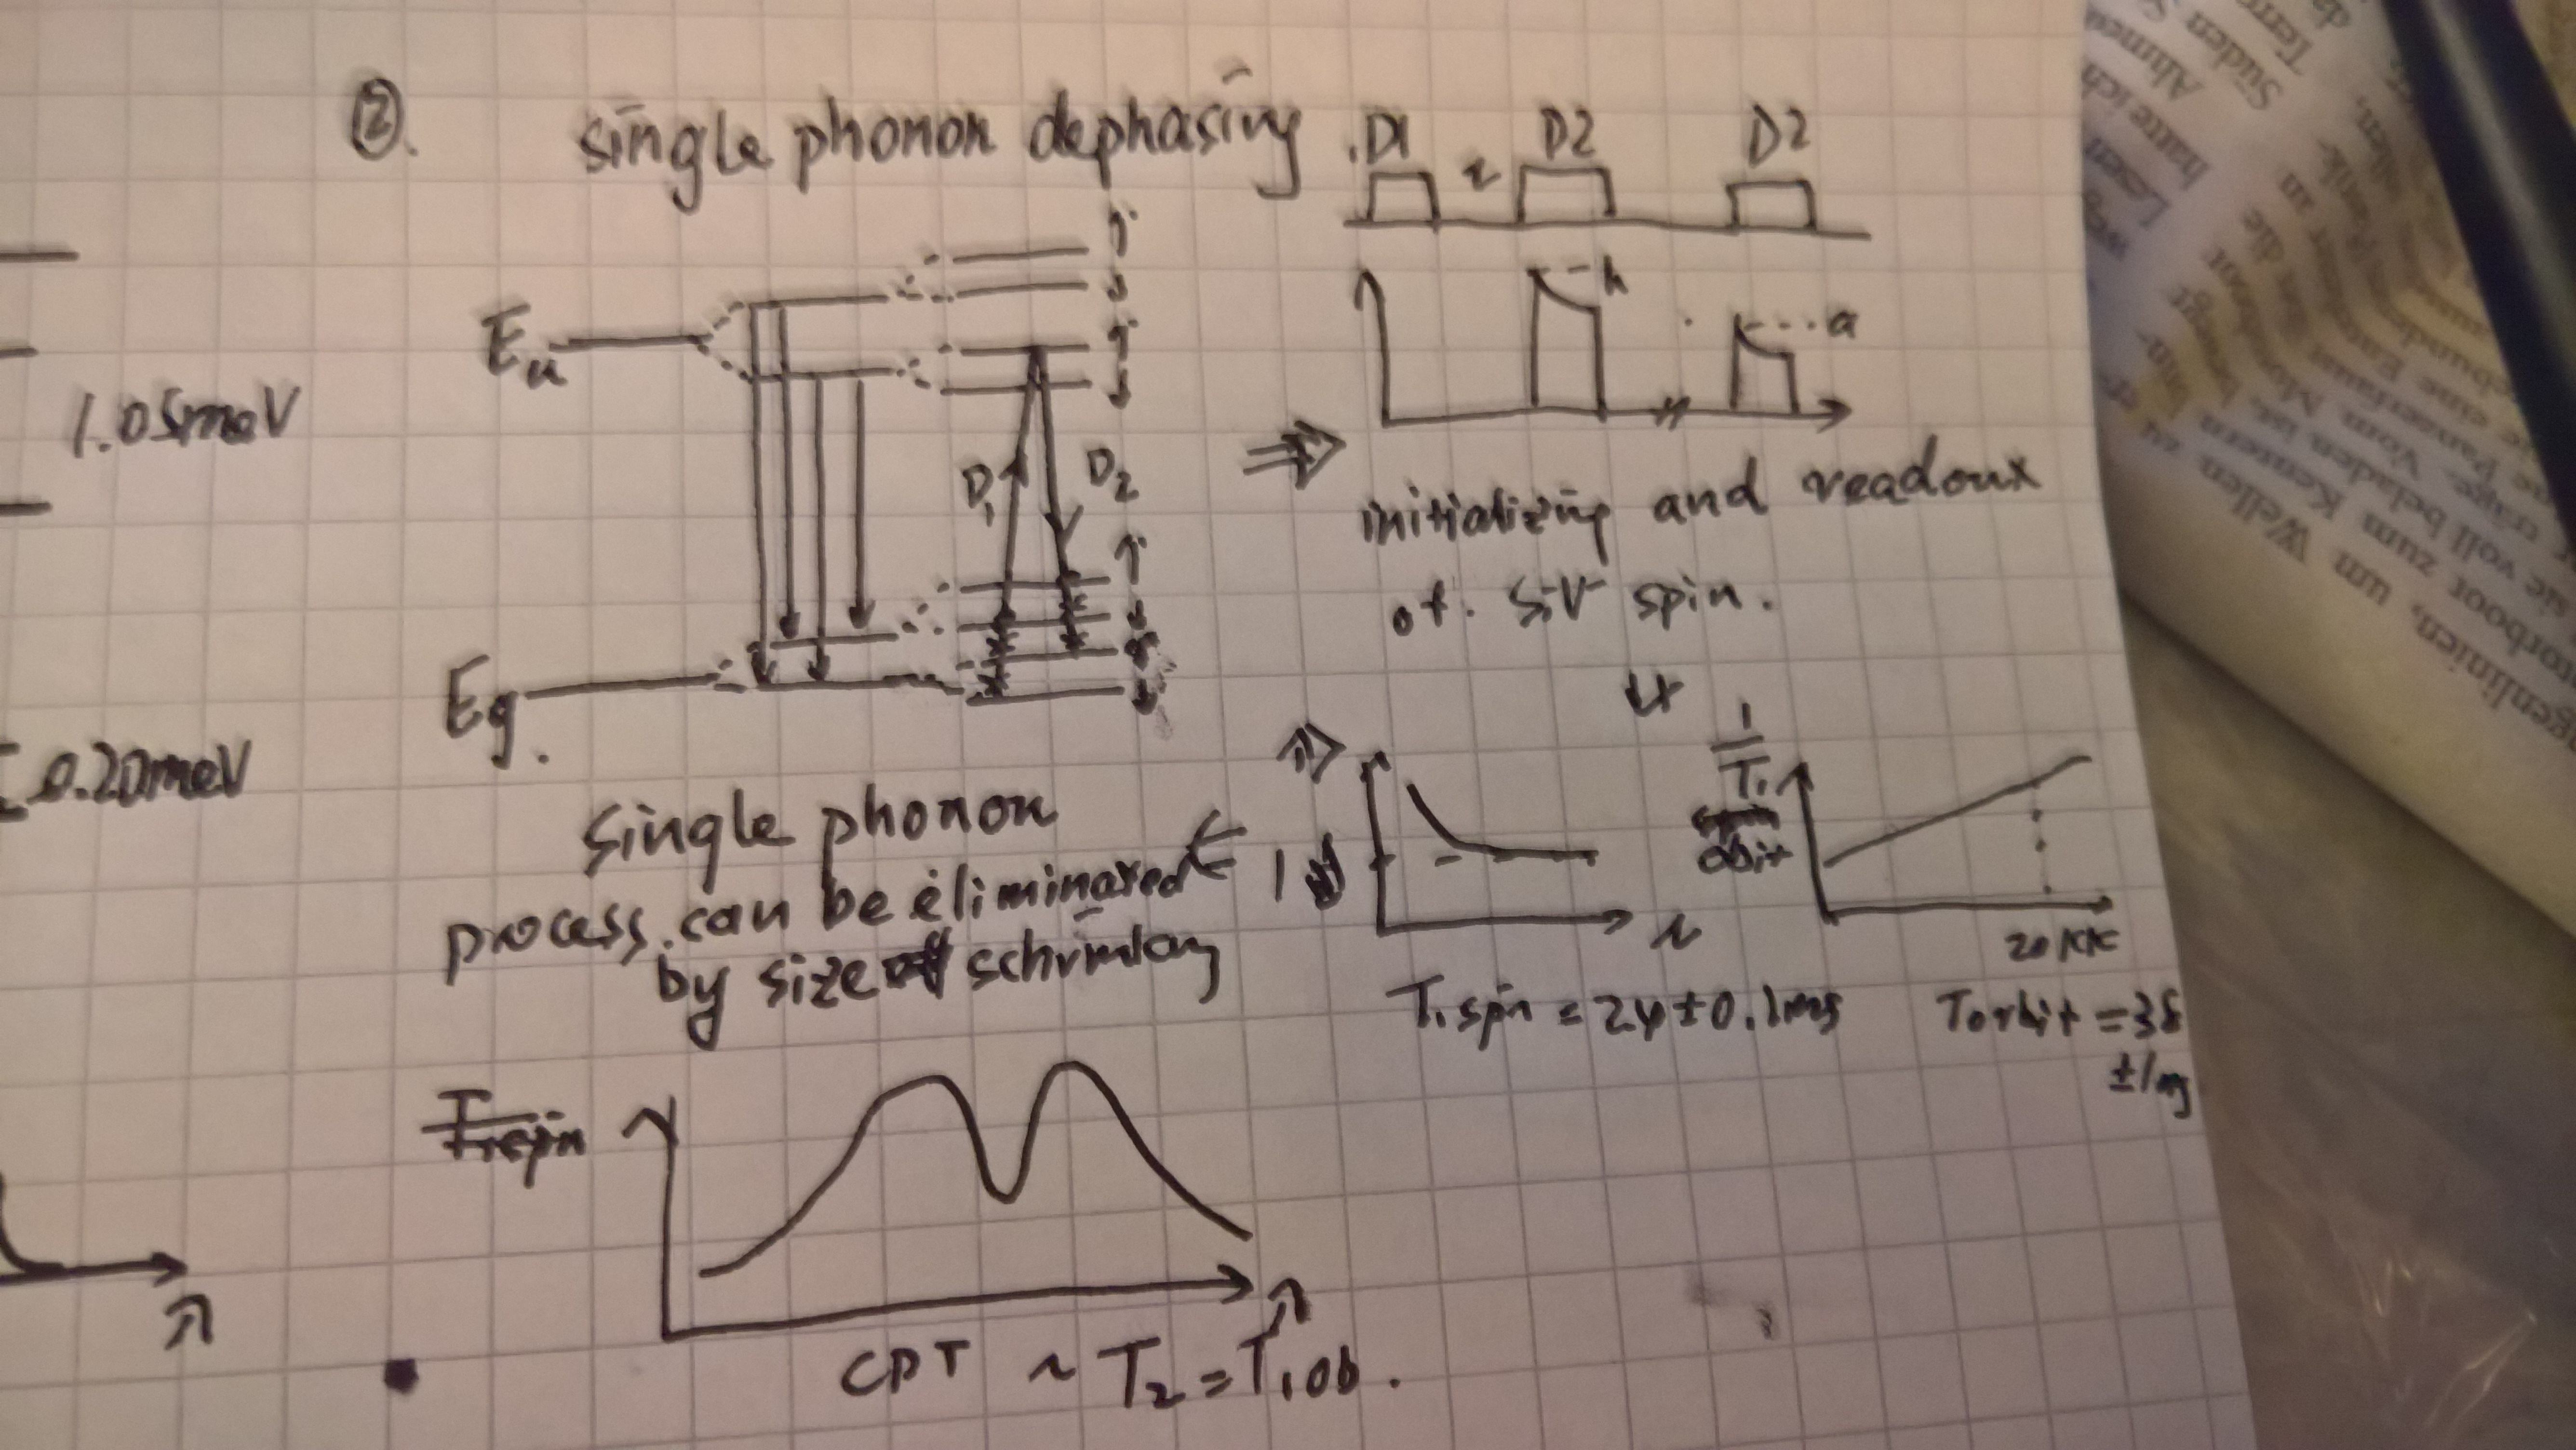
\includegraphics[width=1\linewidth]{Figures/pic/WP_20160921_20_40_32_Pro_LI}
\caption{}
\label{fig:wp20160921204032proli}
\end{figure}
\FloatBarrier

%----------------------------------------------------------------------------------------

\section[Silicon vacancies in nanodiamonds]{Silicon vacancies in nanodiamonds}
\FloatBarrier
\begin{figure}[h]
\centering
\includegraphics[width=1\linewidth]{Figures/pic/WP_20160921_20_40_48_Pro_LI}
\caption{}
\label{fig:wp20160921204048proli}
\end{figure}
\FloatBarrier
As mentioned, one vital problem to solve if we want to use SiV$^{-}$ as a qubit is that, the coherent time has been limited by the rapid orbital relaxation. And this is caused by the transition between the degeneracies of ground state which was driven by a single phonon. The elimination of such phonon is an direct approach towards the solution.

Spontaneous emission is inhibited if the cavity has characteristic dimensions which are small compared to the radiation wavelength [Daniel Kleppner1981]. As in our case to eliminate the emission of phonon that couples into the splitting of ground state in SiV$^{-}$ 47 GHz, nanodiamond of the size that is smaller than the half wavelength of this transition phonon wavelength (around 125nm) is desired. 

Currently 3 major techniques are employed in the field of nanodiamond fabrication: denotation, CVD, and HPHT, while the exotic atoms can be mixed in the beginning or implanted via ion implantation. While the denotation method produced highly defective diamonds and ion implantation introduces inner strain, for the SiV containing nanodiamonds, HPHT method and CVD method are the top choices.

The principle of CVD method is to disintegrate the CVD fabricated diamond film, while the HPHT method initialize an phase transition of carbon at high temperature and high pressure. Previously, comparison between the PL spectra of silicon doped polycrystalline diamond films obtained by the CVD method and diamond single crystals grown at a pressure of 6 GPa from a nickel melt at 1500$^{o}C$ has been carried out, and demonstrates that the HPHT diamonds carries narrower SiV$^{-}$ ZPL lines than CVD fabricated ones[C. D. Clark 1995]. As in the department of nanodiamonds, the narrowest SiV$^{-}$ ZPL that has been measued by far, which has the width that is almost of the excitation state life time limit, is also from the HPHT method fabricated nanodiamond.


 
\paragraph{Band-bending near the surface of diamond}  


%--------------------------------------------------------------------------------------

\section[Motivation of the thesis, unsolved problem]{Motivation of the thesis, unsolved problem}
\FloatBarrier
\begin{figure}[h]
	\centering
	\includegraphics[width=1\linewidth]{Figures/pic/WP_20160921_20_40_42_Pro_LI}
	\caption{}
	\label{fig:wp20160921204042proli}
\end{figure}
\FloatBarrier
The motivation of looking into SiV$^{-}$ in nanodiamonds is to acquire longer coherent time by eliminating the phonon that is responsible for the transition between the fine splitting of the ground state. Yet the obstacle on our way of justifying this approach is that, the optical properties of SiV$^{-}$ in nanodiamonds are not as outstanding as it is in bulk diamond. Blinking and spectral diffusion, especially spectral diffusion has stopped us from further life time measurement. 

The mechanism behind the spectral diffusion is yet not clear, our first guess is to connect the enhancement of spectral diffusion in nanodiamonds with the surface condition, due to the high surface to volume ratio of nanodiamonds.

Aerobatic oxidation can purify the nanodiamonds via the removal of Sp$^{2}$ phased carbon.
% Chapter 2
\chapter[Experimental approach of surpressing the spectral diffusion]{Experimental approach of surpressing the spectral diffusion} % Main chapter title

\label{Chapter2} % Change X to a consecutive number; for referencing this chapter elsewhere, use \ref{ChapterX}

%----------------------------------------------------------------------------------------
%	SECTION 1
%----------------------------------------------------------------------------------------
\section{Information regarding the nanodiamond sample}

\paragraph{here is a paragraph about the fabrication of nanodiamond}
\paragraph{here is a paragraph about the separation of the nanodiamonds}
\section[sample preparation]{sample preparation}
\subsection{preparation of the substrate}
\paragraph{IIa diamond as substrate}

To choose a proper substrate for the nanodiamond sample, a few principles need to be considered.

\paragraph{1.}Low background fluorescence. 
It is always vital to obtain a decent signal to noise ration in any kind of meansurements. As for our case, the emission(fluorescence) from sillicon centers are the target, thus we would love to lower the back ground fluorescence as much as possilble.
\paragraph{2.}Good heat conductivity at low temperature.
From previous calculation done by Uwen Jantzen, we know that the temperature difference $\bigtriangleup T$ between the bottom of the substrate and nanodiamonds(which are spin coated on the surface of the substrate) can be estimate as\newline
$\bigtriangleup T = \frac{\sigma \cdot d \cdot T^{4}}{k} $,
where $\sigma$ is the Stefan–Boltzmann constant, $d$ is the thickness of the substrate and $k$ is the thermal conductivity.
To resolve the fine feature of sillicon vacancy ZPL, we want to characterise the nanodiamond sample at a temperature that is lower than 30K for spectrometer and 10K? for PLE.
\paragraph{3.} No distracting spectral features.
Some misleading peaks from the emission of the substrate would be the least wanted when we want to character a sample spectrally. In many cases, this is related to the raman-scattering of the photons, which highly depends on the crystal structure of the substrate. This scattering process alters the energy of the incident photons by shifts of concrete values and sometime can introduce peaks that are misleading or distracting.
\paragraph{4.}Refractive index. Inam et al calculated the relative emission rate for radiating dipoles near an interface between two dielectrics with FDTD simulation. The result demonstrates that in both of the cases, when the dipole lies prependicular and parallel to the substrate, the emission rate from a interface with lower relative refractive index is always higher than that from a interface with higher relative refractive index. And to increase the emission rate, a substrate with lower refractive index would be prefered.
\paragraph{}Prevously, taking these principles into consideration, my colleges have already ruled out a couple of materials, for instance, glass/quartz(distraction raman shift lines) and Sapphire(also a distracting raman shift line, and impurity induced emission that calls for extra attention when picking the optical filters). Now the temporary choice has landed on IIa type diamond, which has a low impurity density(resulting in low background fluorescence intensity), relatively low refractive index(2,4 to 2,7), good thermal conductivity($\bigtriangleup T = 4,17 \cdot 10^{-2}K$) and a raman shift at 1332$cm^{-1} $ that causes no distraction on our observation.

\paragraph{Focused Ion Beam milling}
In order to make it more convenient to trace the nanodiamonds, markers were curved onto the surface of the IIa type diamond substrate, this work was done by Uwe Jantzen during his master's thesis period. As is shown in the fig.[], the focues ion beam bombards the surface of diamond away and leaves behind markers that are visible in optical microscopy images and SEM images, as well as confocal microscopy images.
\paragraph{here is a sketch of how Ga-ion bombards the surface of substrate}
\paragraph{here insert image of markers, optical, sem and confocal}
\paragraph{fig. ?.  }



\subsection{spin-coating of the sample}
\subsubsection{theory of spin coating} 
Spin coating is the method of sample preparing that mainly contains 2 steps:

1. Spreading of the liquid. In this step, certain volume of liquid containing the particle that we want to coat with is dropped on the surface of the substrate, driven by the centrifuging force from the rotational movement of the substrate, the liquid would be spread evenly on the surface.

2. Evaporation of the 'solvent'. While the sample stage rotates, the 'solvent'(In our case is not a real solvent, since nanodiamonds never really desolve.) would evaporate, leaving the particle/molecules that are wanted to be coated on the substrate.

In this procedure, 2 factors we find important.

1.spin speed: generally the thickness of the liquid layer $t$ is proportional to the inverse of the angular velocity $w$ squared t $\sim$ $\frac{1}{\sqrt{\omega}}$, higher speed would help with forming a more uniform layer, yet this also means a smaller volume of solution, which would lead to lower density of nanodiamonds of the surface. On the other hand, with lower speed, the probability of aggregation would increase, which is also what we want to prevent.

2.volume of the 'solution': larger volume means longer drying time, which would increase the probability of aggregation and losing nanodiamonds, while smaller volume leads towards lower density of nanodiamond and more difficulty when trying to drop it with a pipette. 

3.type of solvent: The type of solvent, viscosity and boiling point are important for the dispersion of nanoparticles inside solution, the spreading of the solution while spin coating and the rate of evaporation.

4.surface condition of the substrate. High contact angle is a obstacle towards the spreading of the solution, high roughness or inappropriate surface group of the substrate can result in poor wettability from the solution.

Throughout my project, with the help of Andrea Kurz, several combination of these factors had been has been tried out and in the end we landed on 

\paragraph{here we need a list of different program of spin coating that we have tried,with indexxxxx}

%-----------------------------------
\subsubsection{Acid cleaning}
To make sure that the NDs dispension can evenly spread and eventually settled on the substrate, a smooth, clean and hydrophilic surface is important.

Acid boiling is a very practicle way of diamond substrate cleaning. As it is called, the diamond will be boiled in a mixture of three strong mineral acids: sulfuric acid, nitric acid and perchloric acid. This mixture has ver strong ability of oxidizing.

\paragraph{here insert a sketch of how we do acid cleaning} 

After assembling the setup, we initialize the reaction by heating the mixture to a temperature where is mildly bubbles. The substrate would be stay inside the boiling tri-acid mix for 4h. 
The mixture of strong mineral oxidizing acid can remove most of the adhesions on the surface of diamond substrate , leaving a clean hydrphilic surface. This oxidizing procedure will lead to the formation of carbonyl and carboxyl groups.




\paragraph {here insert image of before and after cleaning substrate, optical image, confocal image }
fig. the comparision between before and after acid boiling.
 
Tri Acid boiling blabla. Expectation of the surface. Before after cleaning. Optical image. Confocal image.

%-----------------------------------
%	SECTION 2
%-----------------------------------
\section[development of a technology to estimate the spectral diffusion]{development of a technology to estimate the spectral diffusion}

\paragraph{Setup} 

In order to resolve the fine structure of ZPL of SiVs, we need to observe the sample at low temperature, thus a cryogenic setup must be applied.
Our setup is a typical confocal micropscopy setup connects with a cryostat, which cools the sample with liquid Helium flow.

\paragraph{here inserts a picture of our flow cryostat, from out and in side.}
This is the flow cryostat, whose main body is a vaccum chamber with

\paragraph{here insert a sketch of the cryo4 setup}
Confocal + Cryostat, Green laser + Red laser, spectrometer, apd, pic


\paragraph{PL} Photoluminescence spectra is one of the most efficient way of finding silicon vacancies. In this measurement, we use green laser of 532nm to excite the Silicon vacancies from ground state to 

\paragraph{PLE} resonance excitation of optical transition. Rsésolution limited by scanning step of laser. Observing phonon side band with apd. range of scanning: limited by laser, small.

\paragraph{time resolved PL spectra} Tracing PL spectra over time, show the diffusing behaviour of lines, characterisation methods: excitation polarisation: width of diffusion. Cross- correlation over time.
\paragraph{}We recorded and noticed that the diffusion, whose range can up to 1nm, is far beyond the capability of PLE. 

%-----------------------------------
%	SECTION 3
%-----------------------------------
\section{Oxidation}
\paragraph{Effect of Oxidation}
Room temperature oxidization is a common way of nanodiamond purification. With different oxidizing temperature, different types of impurities can be removed from the surface of the nanodiamond, ranging from water and physisorbed organic impurities, amourphous carbon, and graphitic shells and ultimate the $sp^{3}$ phase of diamond[T.Gaebel,2010]. After the oxidation, carbonyl and carboxyl groups are formed on the surface[Petrakov,2012]. Several paper have mentioned temperature choices for oxidation aiming at impurity removal. During the master's thesis period, 2 different oxidation has been examined.

\subsection[first Oxidation]{first Oxidation}
\paragraph{method}As reported, oxidation of $sp^{2}$ carbon already starts at $400^{o}C$, while the size reducing rate of diamond phase remains neglactable when the temperature is lower than $500^{o}C$. So it is an obvious choice to settle down the oxidation temperature at somewhere close to $500^{o}C$ when the maximum removal of $sp^{2}$ phased carbons and the minimum lost of the diamond body($sp^{3}$ phased carbons). Inspired by Elka Neu's paper, ....here insert a sentence explaining why we choose the two step oxidation program.
\paragraph{setup}

The aerobatic oxidation is carried out in a tube furnace that is offered by the ?? institute and it is done with the help of Markus Mohr. The tube furnace consists of a glass tube connected to the room atmosphere and heating coils around the glass tube. The glass tube is slidable. We put our sample inside a ceramic ?bowl? and put the bowl into the glass tube carefully, after the temperature has been raised to ?460C?, the glass tube would be slide into the heating coils. After the Oxidation, the glass tube would be slide out and the sample would cooled inside the tube until room temperature.

\paragraph{pre-characterisation}
Before the oxidation, we tried to characterise the sample with several different methods based on our confocal microscopy setup.

1. RT imaging and PL spectra

First we take a scan with green laser and record the fluorescence with an APD, which offers us a confocal microscopy image of the surface of the sample, then the photoluminescnce spectra of the bright spots are taken, those ones with a sharp peak at 737nm are saved as points of interests and their positions are saved as region of interest for the reference of further examine.

2. Cold spectra and PLE 
The sample is attached to an cold finger and the placed inside the cryostat, after UHV condition has been achieved, we start the helium transfer, which would brought the temperature of the sample down to 4.8K. We refound the points of interests that has been confirmed with SiV like spectra

3. PLE spectra

4.time-resolved PL spectra.

\paragraph{post-oxidation characterisation}
1. Optical microscopy check
The first thing we found after the oxidation is that, the surface of our sample turned very dirty. We are yet not certain about what the contaminations are, are they intrinsic or are they external. A possible deduction is that, the contamination comes from the glass tube of tube furnace, that the residues of previous treatments has attached to the inner surface of the tube and evaporized again, depositing on the surface of our sample. Further improvement of oxidation operation has been done in our second oxidation test, and will be mentioned in the next part of the thesis.


2. confocal microscopy imaging and PL spectra.
Huge amount of bright spots can be seen in the confocal image when we excite the sample with 532nm green laser. There's no Silicon vacancy like spectra found in these bright spots. We refind our points of interests next to the marker 4C. The photoluminescence spectra shows much higher intensity than before the oxidation.


3. Cold spectra and PLE 
After the confirmation of points of interests, the sample was transfered into the flow cryostat and the helium flow brought the temperature down to 4.8K.

At 4.8K we recorded the time-resolved photoluminescence spectra of different incident beam power with an excitation wavelength of 532nm. 

After the first oxidation, we learned that due to the inner strain of photonic fibre, the incident beam can not preserve a static polarisation. To stable the polarisation, we used a polarising beam spliter with a LC noise eater behind it. This would fix the polarisation at vertical direction.


\paragraph{Analysis}

\subsection[Second Oxidation]{second Oxidation}

\paragraph{method} As is mentioned before, the optical properties of SiV in bulk diamond is extraordinary. Most importantly, the spectrodiffusion that we have observed in nanodiamonds has never been seen in bulk diamonds. In the first oxidation, it seems the removal of graphitic impurity didn't help with the stablization of emiision lines. In this second oxidation, we decided to used a higher temperature to acquire a surface with groups that imitates the bulk diamond.As reported by [paper], after 2 hours of aerobatic oxidation at $575^{o}C$, ... here insert a sentence of the surface groups of nanodiamonds. To increase the chance of finding smaller nanodiamonds that would fit into a cavity and decrease the chance of getting clusters of nanodiamonds, this time we chose to use nanodiamond of the first batch. These nanodiamond are spin coated on the substrate following the method II(the index, can be change).

Taking the experiences of last oxidation into consideration. This time we introduces flowing inert gas (helium) to flush away the potential contaminations during the cooling process. This can also prevent the result to be affected by the humidity of the air.
We found out the extinction rate of polarising beam spliter is not ideal, so this time we used a Clan Thompson polarisation filter instead.
\paragraph{Before Oxidation}
1.Optical microscopy observation
  
We observed the sample after the spin coating with optical microscopy, the surface appeared to be relatively clean, little amount of contamination has been observed, but is acceptable.

2.Mapping of $SiV^{-}$ with room temperature setup.

Once again, we exxplored the sample with the same room temperature confocal microscopy setup. With the help of spectrometer, we find a few points of interest with a emission spectrum that resembles $SiV^{-}$. 

3. Cold time resolved PL and exitation polarisation

As has been mention in last chapter, it is suspect that the incident polarisation can affect the spectral behaviour of SiV. We added in the excitation polarisation measurement and recorded the time resolved photoluminescence spectra of 2 different excitation polarisation that are perpendicular to each other. This is achieved by putting a motor-driven half-lambda plate after the noise eater. 
Due to short time scheme from this measurement we decided to fix the input power at [?need to check], which is the lowest power that can offer most of the points of interest's a decent signal to noise ration.




\paragraph{After Oxidation} 

1. Optical Microscopy observation. 

After the Oxidation, we found the surface not as dirty as the last Oxidation. It seems a cleaner tube and flowing gas flushing do have helped suppressing the surface contamination introduced by the tube furnace.



\paragraph{Analysis} 
Comparasion if possible: different behaviour pre treatment between two batches
Possible reason: losing NDs due to Helium flow while cooling, GR1 getting closer to the surface due to oxidation caused size/thickness reduction.

%----------------------------------------------------------------------------------------
%	SECTION 4
%----------------------------------------------------------------------------------------

\section[H termination]{H termination}
\paragraph{Effect of H termination}

NEA, band structure of diamond. Reduction of surface.
\paragraph{method} Plasma treatment, setup, apparatus.

\paragraph{why no pre characterisation} Conditions for Plasma treatment.

\paragraph{After H termination} Confocal image, optical image, excitation polarisation, time resolved PL with different incident polarisation.


\paragraph{Analysis} Within the instrumental limit of spectrometer, the spectral diffusion has been significantly suppressed. Possible reason. 

\chapter{Surface treatments} % Main chapter title

\label{Chapter2.5} % Change X to a consecutive number; for referencing this chapter else where, use \ref{ChapterX}



%-----------------------------------
%	SECTION 3
%-----------------------------------
\section{Oxidation}
Room temperature oxidization is a common way of nanodiamond purification. With different oxidizing temperature, different types of impurities can be removed from the surface of the nanodiamond, ranging from water and physisorbed organic impurities, amourphous carbon, and graphitic shells and ultimate the $sp^{3}$ phase of diamond[T.Gaebel,2010]. After the oxidation, carbonyl and carboxyl groups are formed on the surface[Petrakov,2012]. Several paper have mentioned temperature choices for oxidation aiming at impurity removal. During the master's thesis period, 2 different oxidation has been examined.

\subsection[first Oxidation]{first Oxidation}
As reported, it is possible to achieve the removal of $sp^{2}$ carbon without any oxidation on $sp^{3}$ carbon via aerobic oxidation with temperature between 375$^{o}C$ and 450$^{o}C$. With temperature lower than 500$^{o}C$, the size reducing rate of nanodiamond is lower than 1nm/h. As our first treatment, we carried out a two step oxidation on sample 1508 and 1509, to achieve the complete removal of graphitic defect on the surface and light oxidation on the surface. Sample 1508 was spin coated with nanodiamond batch2, sample 1509 was spin coated with nanodiamond batch1.

The aerobatic oxidation is carried out in a tube furnace and it is done with the help of Markus Mohr. The tube furnace consists of a glass tube connected to the room atmosphere and heating coils around the glass tube. The glass tube can be slide in or out of the heating coils. We put our sample inside a ceramic sample holder and put the holder into the glass tube carefully, after the temperature has been raised to 460$^{o}C$, the glass tube was slide into the heating coils. The sample was oxidized at 460$^{o}C$ for 90min,then 480$^{o}C$ for 40min. After the Oxidation, the glass tube was slide out and the sample stayed inside the tube until it reached room temperature.

Before the oxidation, the samples was first mapped with a room temperature setup that resembles fig. 2.4, but without vaccum pump and cryostat. To make a map of SiV$^{-}$ containing points of interest, it was first taken, a scan with green laser while the fluorescence was recorded by APD, which offers us a confocal microscopy image of the sample, then the photoluminescnce spectra of the bright spots were taken, coordinates of those ones with a sharp peak at 737nm saved as points of interests for the reference of further examine.

\begin{figure}[h]
\centering
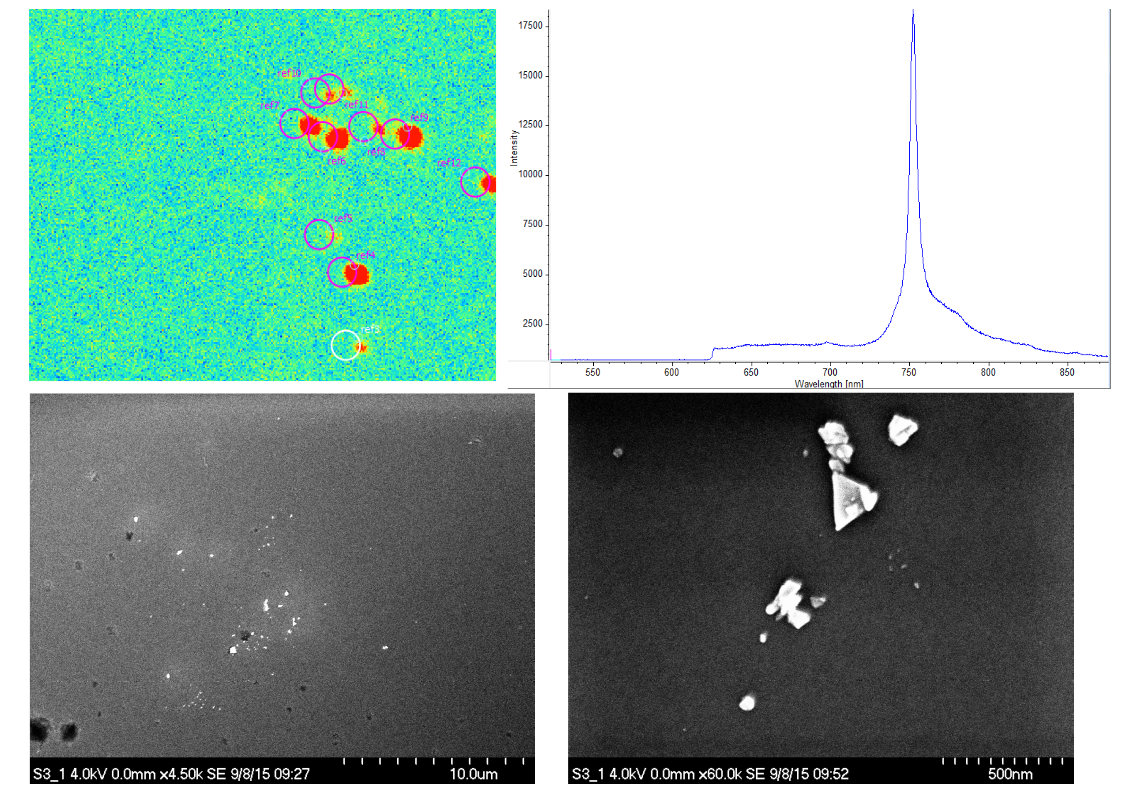
\includegraphics[width=1\linewidth]{Figures/pic/RTPL}
\caption{A)confocal image of a region of interest. The bright spots with circle markers are points of interest. B)Room temperature spectrum of a poi recorded by spectrometer. C)the roi in SEM. D)ref10 and 11 in SEM.}
\label{fig:2015-09-07-ow-capture-20150907151210-744-1}
\end{figure}

Once the map was acquired, we bring the samples to the electron microscope center and observed the regions of interest with SEM. SEM showed that, sample1508 contains more big single crystals that are larger than 300nm and clusters, while sample 1509 contains more single crystal with under 200nm sizes. This proved that the size selection via centrifuging has worked.
 
The samples was then attached to an cold finger and the placed inside the cryostat, after UHV condition has been achieved, the helium transfer was started, which would brought the temperature of the sample down to 4.8K. Most of the mapped pois are refound. Excitation with 532nm green laser double checked the existence of SiV. After the confirmation, it has been tried to carry out a resonance excitation with Titan Sapphire laser, when observing a few points of interest next to marker 5A in sample1509, it was noticed that while scanning the red laser across the line with the help of very low amount of 532nm for repopulation, a spectral diffusion of 6GHz in 15Min has been observed. To exclude the possibility of instrumental error, PLE has been operated on the bulk diamond sample with also SiV inside, where no spectral diffusio has been observed(Fig. 3.2). It has also been noticed that the increase of green laser power can cause more severe spectral drift/jump. In a case when the power green laser is brought up for a better refocus, the line has shifted totally out of the range of the spectra scan, and didn't recover in 10min. This observation brought difficulty in the measurement of orbital T1, since we always need to initialize the obital states with green laser, and this spectral diffusion that is related to the application of green laser can result in the fail of hitting the resonant wavelength, since it is technically difficult to refind the line and adjust the wavelength of the resonance laser coordinately. 

\begin{figure}[h]
\centering
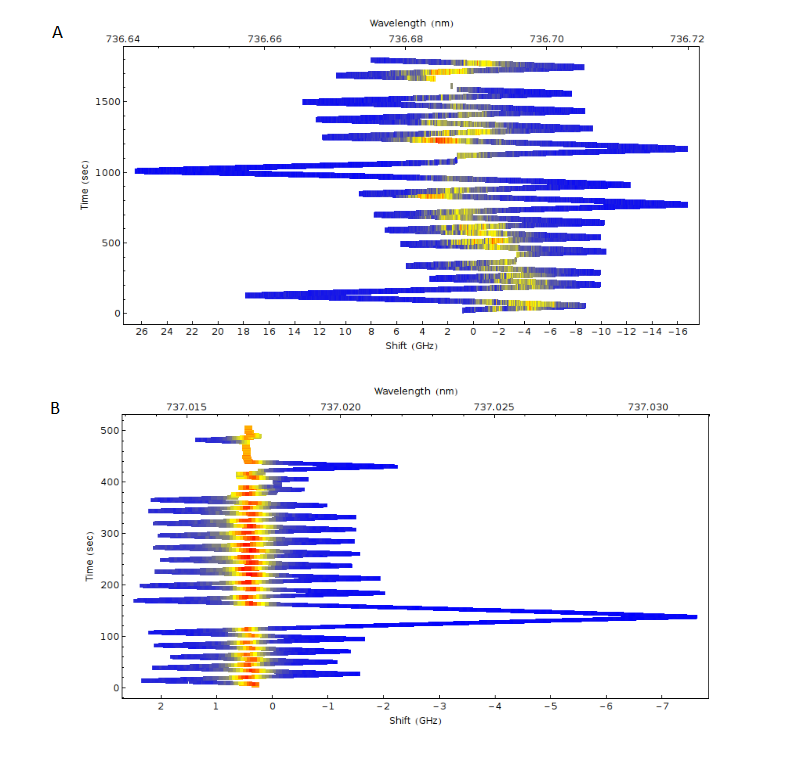
\includegraphics[width=0.7\linewidth]{Figures/pic/PLE}
\caption{PLE scan over time on A) ref5A$\textunderscore$014 from sample1509 and B) a SiV$^{-}$ site from bulk diamond sample 33b. No significant spectral diffusion been found in bulk diamond sample, which exclude the possibility of instrumental error.}
\label{fig:ple}
\end{figure}

After the obeservation above, we want to study more about this spectral diffusion behaviour that is associated with the green laser. We noticed that the sudden jump/diffusion when more green power is applied can be larger than 20GHz, maybe it is easier to track the movement of the lines with the high resolution grating of spectrometer than with PLE.

To observe the diffusion with a spectrometer, we introduced time-resolved photoluminescen spectrum, which has been described in last chapter. Due to the technical problem, our motorized sample stage can not move ideally in the vertical direction anymore, which has limited our region of observation. This time we refound the ROI around the marker 4C. And recorded the time-resolved spectrum. A session is set to be 60 spectra taken consecutively. At first, to feel the long term diffusing better, 3 sessions, with a refocus after each, are undergone for each points of interests. Since line diffusion in PLE gets wider when raising the green laser power, we excite the sample with 500uW power in front of the objective lens to obtain more diffusion. As a result, line diffusion up to 1nm has been observed.Sequentially we decrease the input power to examine the power dependency of spectral

Taking the samples out of the furnace, we noticed that the surfaces of the samples turned very dirty. It is yet not clear, what the contaminations are, are they intrinsic or are they extrinsic. A possible explanation is that, the contamination comes from the glass tube of tube furnace, that the residues of previous treatments has attached to the inner surface of the tube and evaporized again, depositing on the surface of our sample. Further improvement of oxidation operation has been done in our second oxidation test, and will be mentioned in the next part of the thesis.
\begin{figure}[h]
\centering
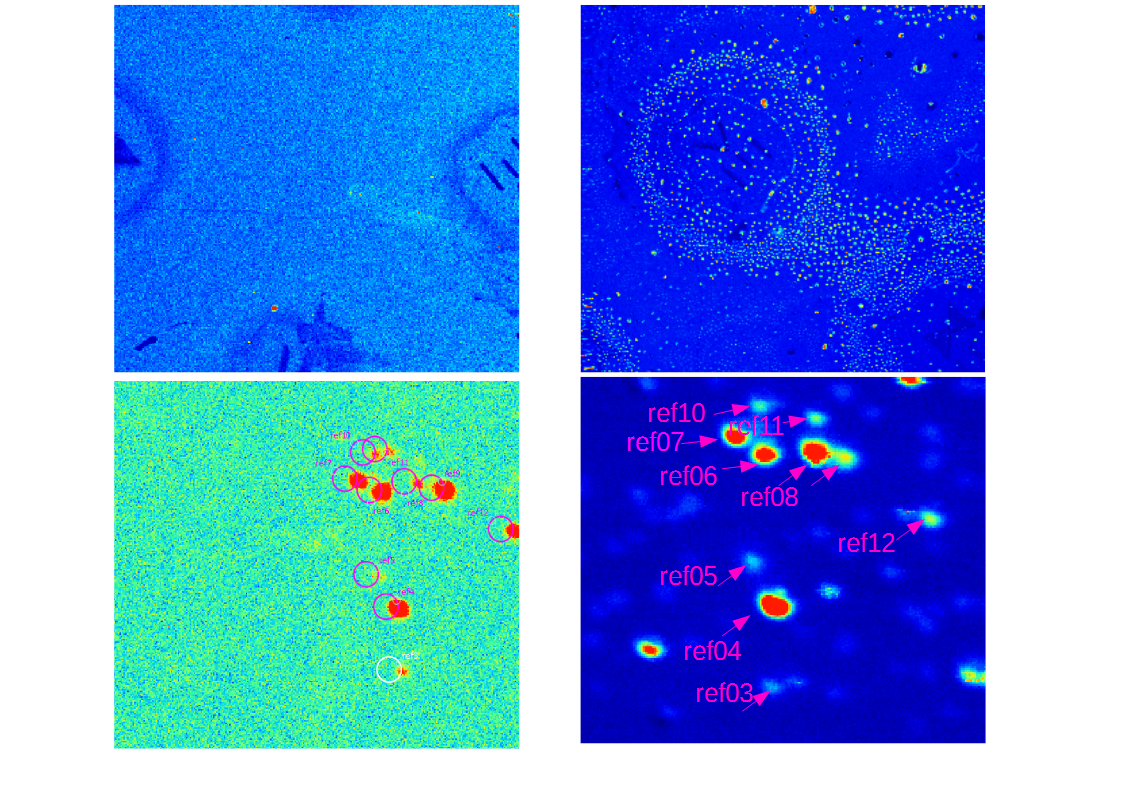
\includegraphics[width=0.7\linewidth]{Figures/pic/oxidation}
\caption{A) region of interest next to marker 3C of sample 1508 before oxidation B)the same region of interest after oxidation C) Points of interest from the ROI before oxidation D)points of interest after oxidation}
\label{fig:oxidation}
\end{figure}

After the oxidation, both of the samples showed very bright background. In sample 1508, large amount of bright spots around the markers has been found. They are not SiV or NV, and will bleach away very fast once been focused on.

I couldn't re-find any marker from sample 1509 due to the large amount of fluorescence from the surface. For sample 1508, the region of interest next to marker 3C was still visible, despite all the disturbing bright spot next to it.

Sample 1509(substrate 207) was then acid cleaned, at the same time sample 1508 was moved into the cryostat, time resolved spectra were recorded. After the oxidation, we learned that the beam polarisation is not conserved within the photonic fibre, so that a polarising beam splitter and a liquid crystal noise eater was added after the fibre to obtain steadily vertically polarised beam. Using the same method as before oxidation, time-resolved PL spectra was recorded.

\subsection[Second Oxidation]{second Oxidation}

The surface function groups play very important role regarding the surface charging state. It is interested to observe, the spectral behaviour of SiV in nanodiamonds, when the surface is initialized the same as bulk diamond. As reported in [Wolcott 2014], after 2 hours of aerobatic oxidation at $575^{o}C$, the surface structure of HPHT NDs is very similar to bulk single crystals where hydroxyl and possibly ethers are the dominant functional groups. It is also interesting, since the elevated oxidation temperature can reduce the size of nanodiamond, to observe the behaviour change as the SiVs will be even closer to the surface after oxidation. Sample 1510 was prepared for this treatment, nanodiamond from batch1 was spin coated on the substrate186$\textunderscore$1 with method IV.

We tried to spin coat substrate 207 at the same time, but failed. The droplet of liquid refuse to spread over the surface while spinning, we suspect the surface of substrate has been damaged in our last oxidation session, which may result in a higher surface roughness that leads to poor wettability.

Taking the experiences of last oxidation into consideration. This time we introduced inert gas (helium) flow to flush away the potential contaminations during the cooling process. This can also prevent the result to be affected by the humidity of the air.
We found out the extinction rate of polarising beam spliter was not ideal for 532nm, so this time we used a Clan Thompson polarisation filter instead.

As mentioned, the polarisation of the beam was not fixed in the measurement before the first oxidation, and while comparing the before and after oxidation spectra, we noticed that, even when the 2 sets of spectra are from the same poi, the spectra pattern can be very different. This made me wonder, if the polarisation of excitation beam has anything to do with the spectral diffusion. To figure this out, we measured the time-resolved PL spectra on 3 pois with different excitation beam polarisation at 4.7K.

The excitation polarisation pattern of other pois are also recorded, but due to low time and Helium budget, it was not affordable to record time resolved excitation polarisation for each of them. Time-resolved PL was later recorded at 20K.

After the oxidation, it was noticed that the sample looks much cleaner than last time. The confocal observation confirmed that, no bright dots like the ones from sample1508 has been seen. The increase of background fluorescence was observed again. Cold spectra showed the existence of GR1 center everywhere.

\begin{figure}[h]
\centering
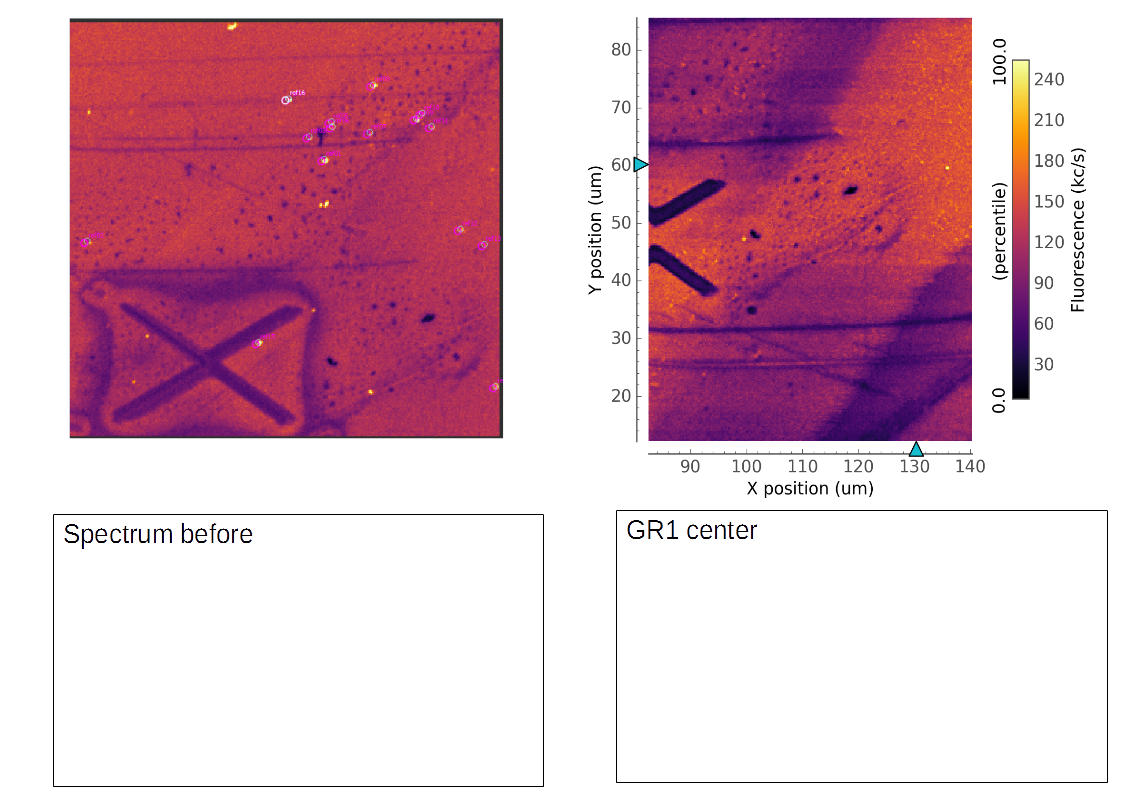
\includegraphics[width=0.7\linewidth]{Figures/pic/afteroxidation2}
\caption{A: roi before oxidation, pois are mapped. B:Background spectrum of the region, no strong Gr1. C:roi after oxidation, strong background fluorescence, can't find pois. D:Spectrum after oxidation, strong GR1 center everywhere.}
\label{fig:wp20160921204221proli}
\end{figure}

I noticed the intensity of GR1 fluorescence is stronger around the FIB made markers. As GR1 centre is a isolated vacancy inside diamond, it is reasonable to suspect that, the impact of focused ion beam may have caused serial collision and collision-induced dislocation inside diamond, resulting in the formation of GR1 centre. The fact that the intensity of GR1 centre is higher after the oxidation can also be explained by this theory, since the cross section is usually of the shape of a droplet, which is larger a few nm beneath the surface that on the surface.

%----------------------------------------------------------------------------------------
%	SECTION 4
%----------------------------------------------------------------------------------------

\section[H termination]{H termination}
As we discussed before, the origin of the band bending is that, the chemical potential of the surface and the bulk region need to match each other, while this adjustment changes the density of charges inside the diamond, it stimulates the generation of space charge, which need to be compensated by the surface charge that is compatible with the shift of the Fermi level from the charge neutrality level (CNL) of the surface state system. The hydrogenate of the diamond surface covers the surface with an atomic layer of $C^{\text{-}} H^{+}$ dipole, which lowers the surface potential, switches the surface from PEA to NEA. I has been experimentally proved that Hydrogenated n-doped diamond has flatter band bending than dehydrogenated ones.[Diederich,1998] 



\FloatBarrier
\begin{figure}[h]
\centering
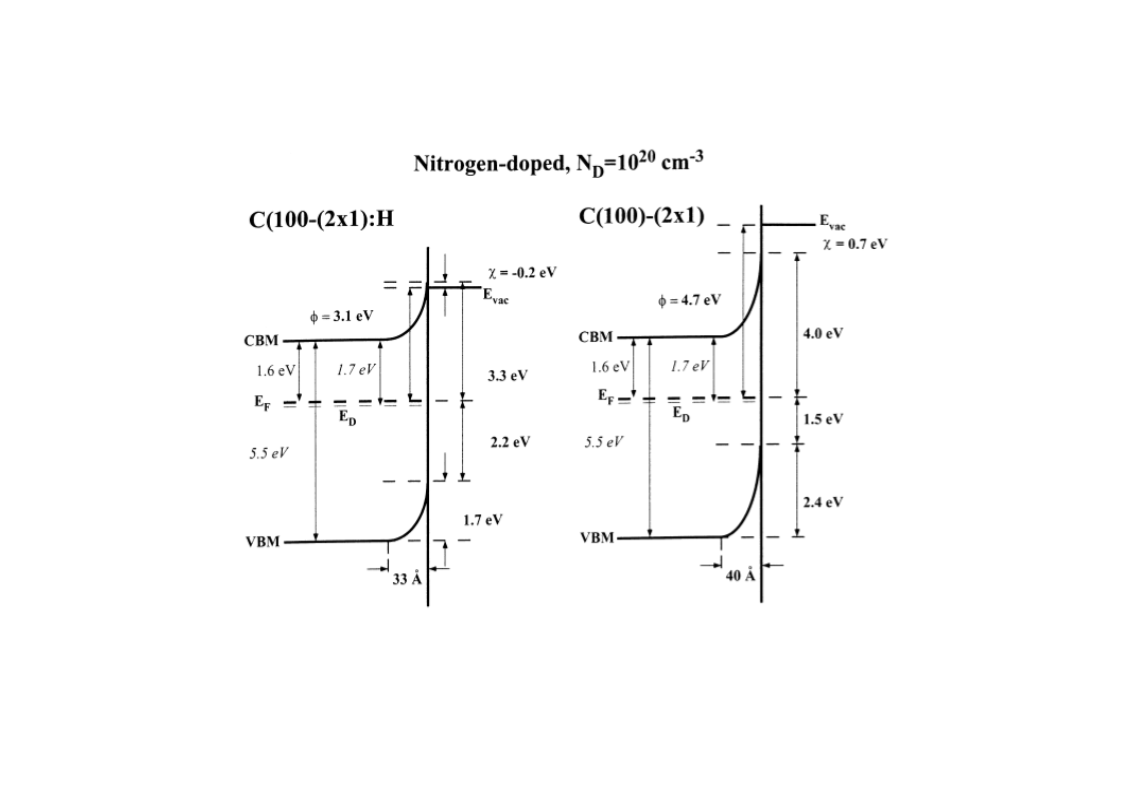
\includegraphics[width=0.7\linewidth]{Figures/pic/Htermination}
\caption{Band structure of N-doped diamond, due to the shift of surface chemical potential, Hydrogenated diamond has flatter band bending than dehydrogenated diamond.[Diederich,1998]}
\label{fig:wp20160921210516proli}
\end{figure}
\FloatBarrier

The surface termination is carried out in a microwave plasma reactor. This is operated by Dr. Christian Osterkamp. We used the same parameters for bulk diamond, (ASK OSCHDI). In [Yeap, 2009], the reaction lasted 60min to maximize the coverage, in our case, considering the low density of nanodiamond on the substrate, we applied the same amount of time as bulk diamond, as the nanodiamond can already be 'dipped' into the plasma thoroughly. The sample that has been used is sample 1512. Sample 1512 was produced by spin coating nanodiamond batch1 on the substrate 186$\textunderscore$2, with method IV.

To prevent introducing contamination into the plasma reactor, no characterisation has been done before the termination. The plasma reactor has the similar vacuum system as a conventional electron microscope, the sample was first put into a pre-vacuum chamber then send into the reaction chamber. The shape of the plasma is controlled by a quartz waveguide. 

After the termination, we put the sample directly into the cryostat, very high density of SiV has been found and marked. It has been recorded as before, the excitation polarisation pattern and the time-resolved PL spectra.
\begin{figure}[h]
\centering
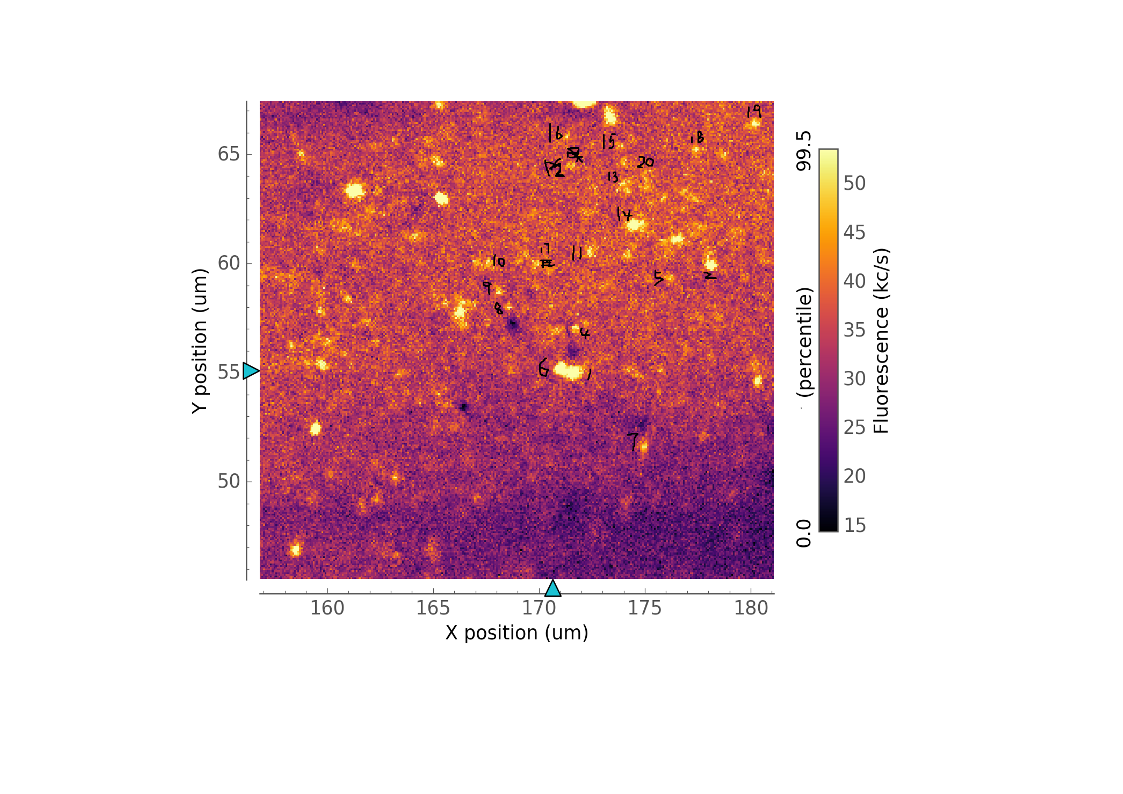
\includegraphics[width=0.7\linewidth]{Figures/pic/hmap}
\caption{Very high density of SiV has been found in sample 1512}
\label{fig:hmap}
\end{figure}


\chapter{Result and Discussion} % Main chapter title

\label{Chapter2.75} % Change X to a consecutive number; for referencing this chapter else where, use \ref{ChapterX}
%----------------------------------------------------------------------------------------
%	SECTION 1
%----------------------------------------------------------------------------------------

%-----------------------------------
%	SECTION 2
%-----------------------------------
\section{Compilation of data}
To investigate the spectral diffusion behaviour, time-resolved spectra were recorded for each of the POI before and after treatment as described in Chapter 3. After the first oxidation, for better characterisation, time-resolved spectra were measured not only with one but multiple excitation polarisation. This leaves large amount of data (almost 32,000 spectra!). Besides visualizing the movement of lines into color maps, we need better tools to evaluate the spectral stability, a way to compile dozens, sometimes even hundreds of spectra into one single value that represents the spectral stability of a POI.

Normalized cross-correlation evaluates the similarity between 2 patterns, the closer to 1, the higher the similarity. Here we compare the time-resolved PL spectra from every time tick with the first spectrum, and the average value of this series of normalized cross-correlation reflects the general level of spectral stability of the measured point.


\section{Nanodiamond size and spectral stability}

The observation of nanodiamond with SEM fits the expectation, that after the centrifuging size selection, batch1 contains smaller nanodiamonds than batch2.  
When comparing the time-resolved spectra from sample1508 and sample1510, which were taken at 4K, with an excitation power of 120$\pm$10uW, it can be observed that the spectra from sample1510 shows more spectral diffusion. The calculation of mean normalized cross-correlation confirmed the observation. As plotted in the histogram \ref{fig:histogram-of-normalized-cross-correlation12}, the distribution of mean normalized cross-correlation for nanodiamonds from batch1 is much closer to 1 than for nanodiamonds from batch2.

\begin{figure}[h]
	\centering
	\includegraphics[width=0.7\linewidth]{"Figures/pic/Histogram of normalized cross-correlation_1_2"}
	\caption{Histogram comparing the normalized mean value of cross-correlation between untreated sample 1508 (nanodiamond batch2) at 4.7K and sample 1510(nanodiamond batch1) at 4.7K and 20K. The height of the bars are normalized by the integration over bins. The time resolved spectra of sample 1510 was recorded with 2 different excitation polarisation, they are separated with solid and dashed lines.}
	\label{fig:histogram-of-normalized-cross-correlation12}
\end{figure}
 


\section{Excitation power and spectral stability}

Sample 1508 was excited with decreasing excitation power. The left column of figure \ref{fig:powerdependenceref11} shows the changes of time-resolved spectra of POI ref11. The most obviously diffusing line is the one between 738nm and 739nm, whose spectral position changed almost 1nm in 300s. As the excitation power decreases, the diffusion become less intense.

\begin{figure}[h]
	\centering
	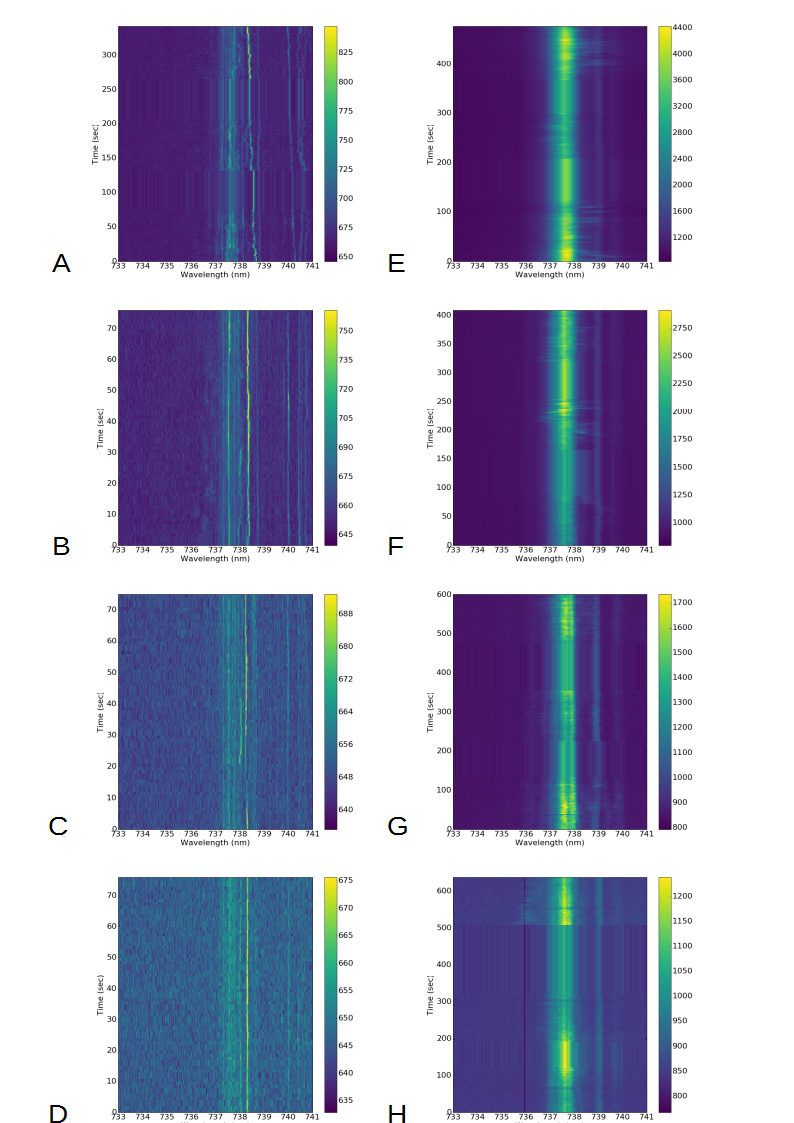
\includegraphics[width=1\linewidth]{Figures/pic/powerdependenceref11}
	\caption{Left column: time resoved PL spectra of point ref11, sample1508 before the first aerobic oxdiation with different excitation power (A:250uW, B:122uW, C:60uW, D:30uW). Right column:time resoved PL spectra of point ref11, sample1508 after the first aerobic oxdiation with different excitation power (A:250uW, B:120uW, C:60uW, D:25uW). The spectra were ploted in the order of real time, the stretched pixel is the blank for refocus.}
	\label{fig:powerdependenceref11}
\end{figure}

The result of cross correlation is can be seen in \ref{fig:powerdependencybeforeafteroxidation}, where each dot represents a POI in the sample. As shown in the figure, the general level of spectral diffusion decreases as the excitation power decreases. 

\begin{figure}[h]
\centering
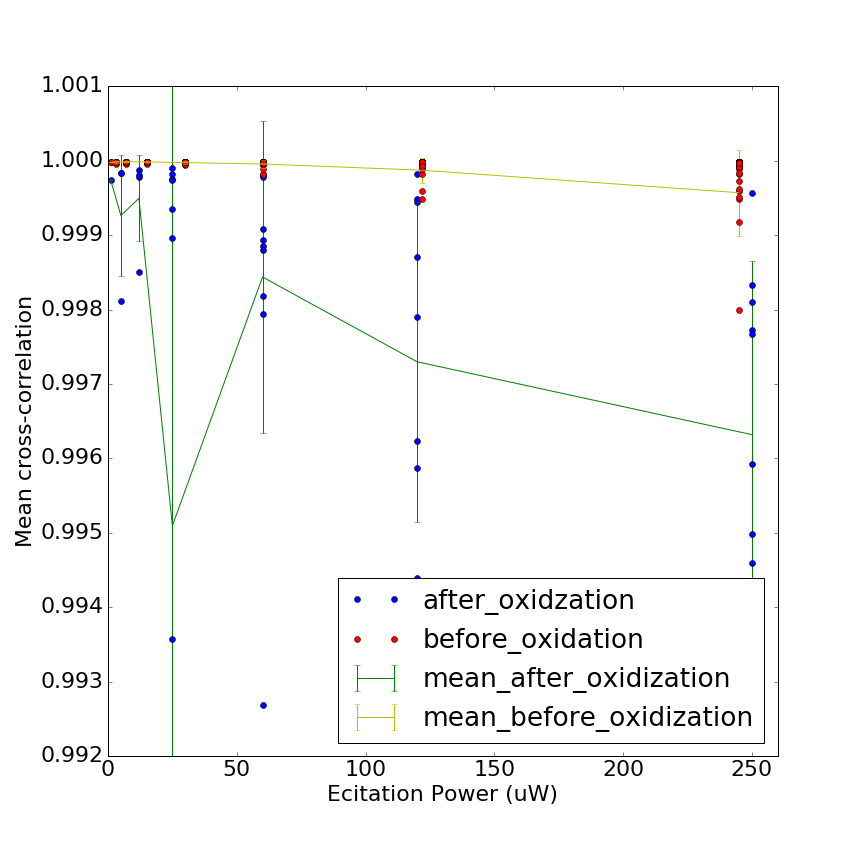
\includegraphics[width=0.7\linewidth]{Figures/pic/powerdependencybeforeafteroxidation}
\caption{Powerdependency of nanodiamond batch2, before and after first oxidation.}
\label{fig:powerdependencybeforeafteroxidation}
\end{figure}

\section{Temperature and spectral stability}
Comparing the mean normalized cross-correlation of sample 1510 from 4.7K and 20K in figure \ref{fig:histogram-of-normalized-cross-correlation12}, no significant difference between the two temperatures has been found, which fits the expectation. Since the assumption is that the donors are ionized with the help of laser, the band bending should stay the same as long as the excitation power is not changed, and therefore so should the spectral diffusion. The result maybe not solid enough as only 3 points were measured for the 4.7K measurement. 

\section{Excitation polarisation and spectral stability}

\begin{figure}[h]
\centering
\includegraphics[width=0.7\linewidth]{"Figures/pic/excitation polarisation"}
\caption{Mean normalized cross-correlation against excitation polarisation. The error bar stand for standard deviation}
\label{fig:excitation-polarisation of untreated nanodiamond batch 2}
\end{figure}

The polarisation of photoluminescence has been measured in \cite{rogers_all-optical_2014}, where the excitation polarisation patterns suggested that the SiV$^{-}$ is aligned along the <111> axis of diamond crystal. The transition have either XY or Z polarisations in the SiV coordinate frame, and so all viewing directions other than along <111> are expected to result in a polarisation dependence for the excitation laser.

In the measurement of excitation polarisation on sample 1510, time-resolved PL spectra are taken with different excitation polarisations. We do noticed some POIs behaved differently when excited with different beam polarisation as shown in figure \ref{fig:polarisationref03}. But no clear polarisation pattern has been acquired. Further cross-correlation calculation was shown in figure \ref{fig:excitation-polarisation of untreated nanodiamond batch 2} showed polarisation dependency like pattern in poi ref12, while the other two pois have no clear pattern.

Further excitation polarisation-resolved spectra were taken on the same sample. In some of the spectra, polarisation-related periodic pattern can be seen on some of the lines, while the sum up pattern give no polarisation dependency.


\begin{figure}[h]
\centering
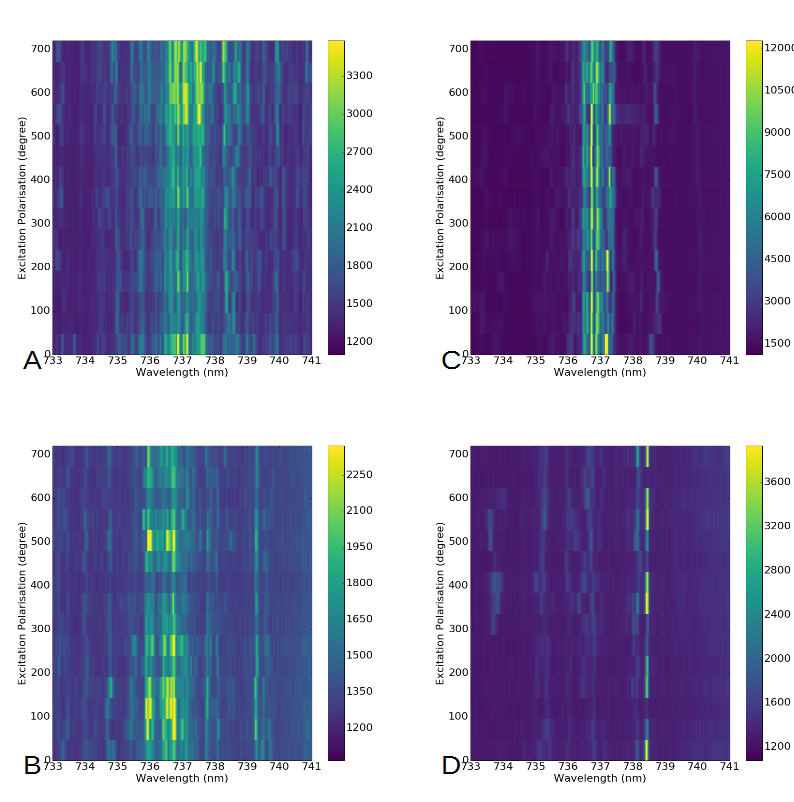
\includegraphics[width=1\linewidth]{Figures/pic/polarisationexcitation}
\caption{4 Excitation polarisation-resolved spectra from sample 1510, A: ref16, B:ref13, C:ref15, D:ref12. Some of the lines in these spectra show polarisation dependency, most significantly can be seen in ref12 }
\label{fig:polarisationexcitation}
\end{figure}
 
\begin{figure}[h]
\centering
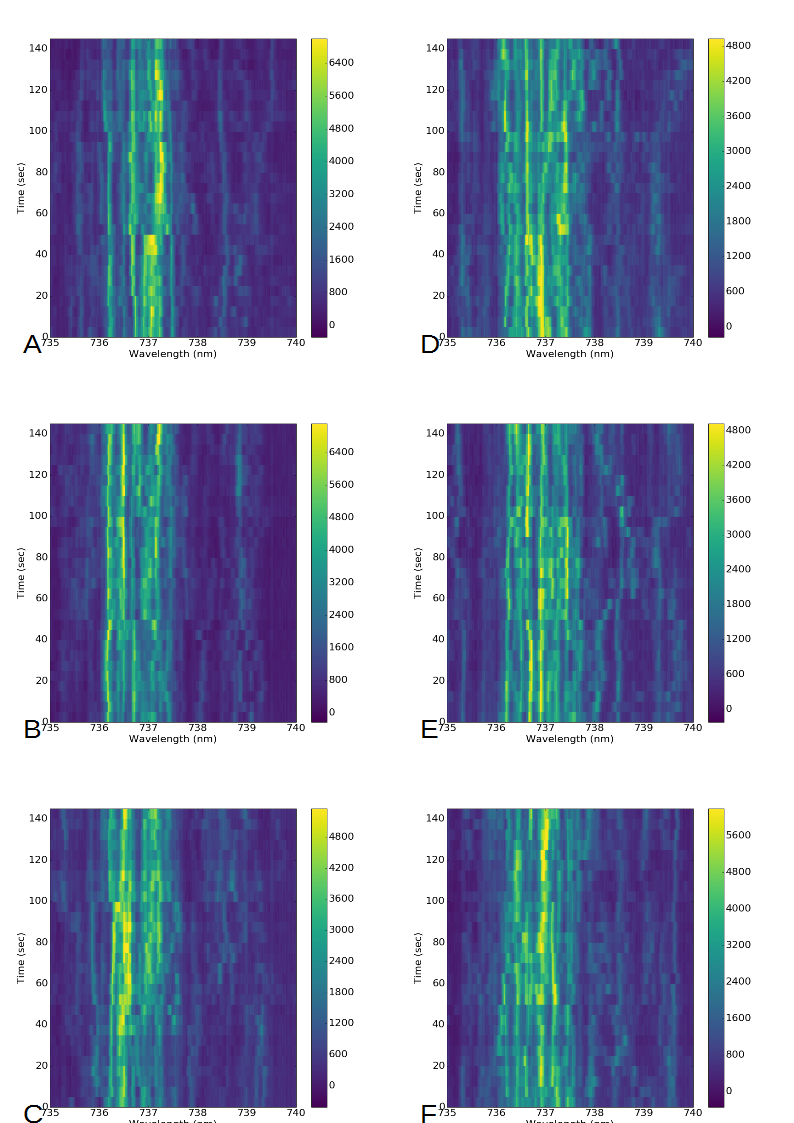
\includegraphics[width=1\linewidth]{Figures/pic/polarisationref03}
\caption{Time-resolved spectra of poi ref03, sample1510 with different excitation polarisation. Polarisation of the excitation beam: A: 0$^{o}$, B: 40$^{o}$, C: 80$^{o}$, D: 120$^{o}$, E: 160$^{o}$, F: 200$^{o}$. This figure continues in \ref{fig:polarisationref032} }
\label{fig:polarisationref03}
\end{figure}
\begin{figure}[h]
\centering
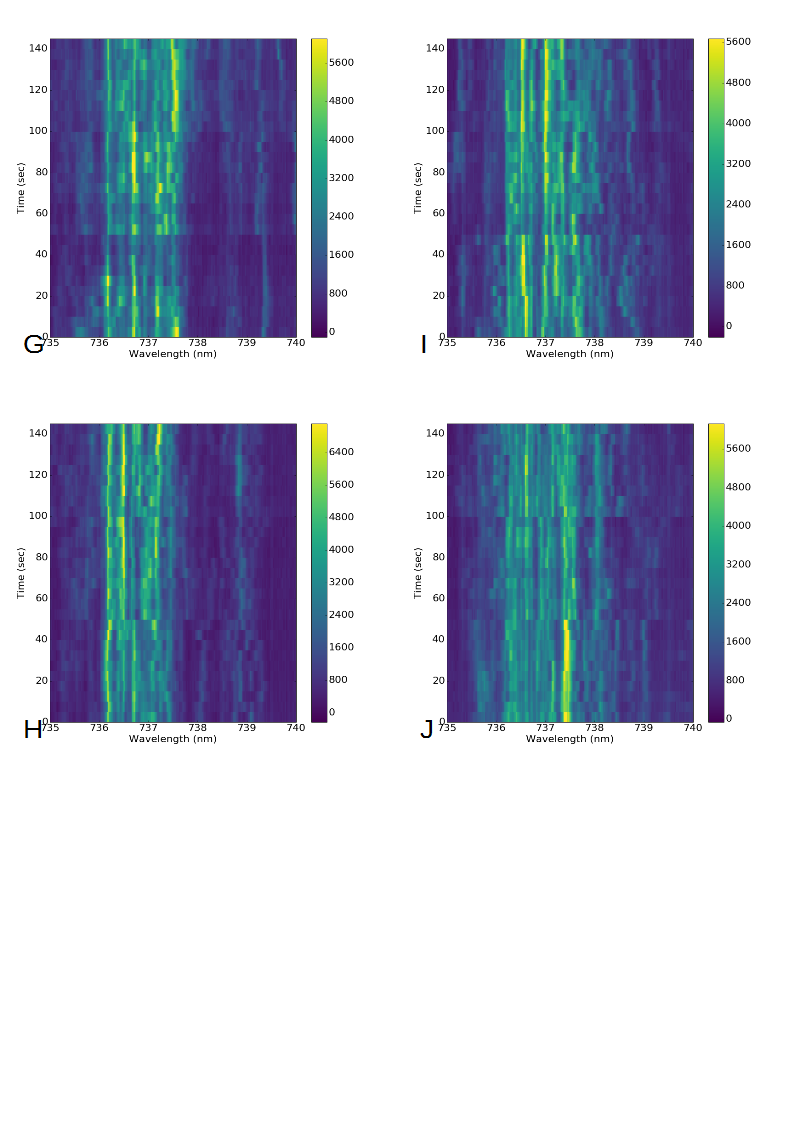
\includegraphics[width=1\linewidth]{Figures/pic/polarisationref03_2}
\caption{This figure follows \ref{fig:polarisationref03}. Excitation Polarisation: G: 240$^{o}$, H: 280$^{o}$, I: 320$^{o}$, J: 360$^{o}$ }
\label{fig:polarisationref032}
\end{figure}







\section{Aerobic Oxidation and Spectral stability}

\paragraph{}The initial target for aerobic oxidation is to selectively remove graphitic defects (the first oxidation) and to generate bulk diamond-like surfaces (the second oxidation). The second oxidation, which was operated on sample 1510, didn't turn out as we expected, offering no useful data on SiV$^{-}$. The first oxidation on sample1508 and 1509 introduced dark spots that are visible in optical microscopy images, and very bright spots containing no SiV$^{-}$ signal in confocal measurements. These are suspected to be exotic, as the furnace has been used for other materials. Yet it was possible to re-find some of the pois from sample1508.

The aerobic oxidation has greatly enhanced the photoluminescence of the sample in general, including SiV$^{-}$ and background. The left column of figure \ref{fig:prepostoxidationspectra} shows the comparison of spectrometer recorded intensity between before and after oxidation, as can be seen in ref3 and other points, the magnification of the enhancement is not uniform. The broadening of peak is also observed. The number of peaks that are distinguishable has decreased after the oxidation. While the spectra before oxidation consists of multiple thinner peaks, the spectra after oxidation contains broader peaks joining with each other. It is suspected that the spectrometer was not well aligned, which results in the broadening of peak  and the disappearance of fine structure. Despite the broadening, an visible enhancement , as shown in figure \ref{fig:prepostoxidationtimeresolvespectra} in the spectral diffusion was also noticed, mean cross-correlation comparison can be found in figure \ref{fig:histogram-of-normalized-cross-correlation2o}. The power dependency of spectral diffusion (mean cross-correlation) is plotted in figure \ref{fig:powerdependencybeforeafteroxidation}, with similar trend as before oxidation: the spectral diffusion increases as excitation power increases. The drop of 30uW is due to an extreme point which obtained very noisy background, that is related to the suspected exotic luminescence from the oxidation process. 

\begin{figure}[h]
	\centering
	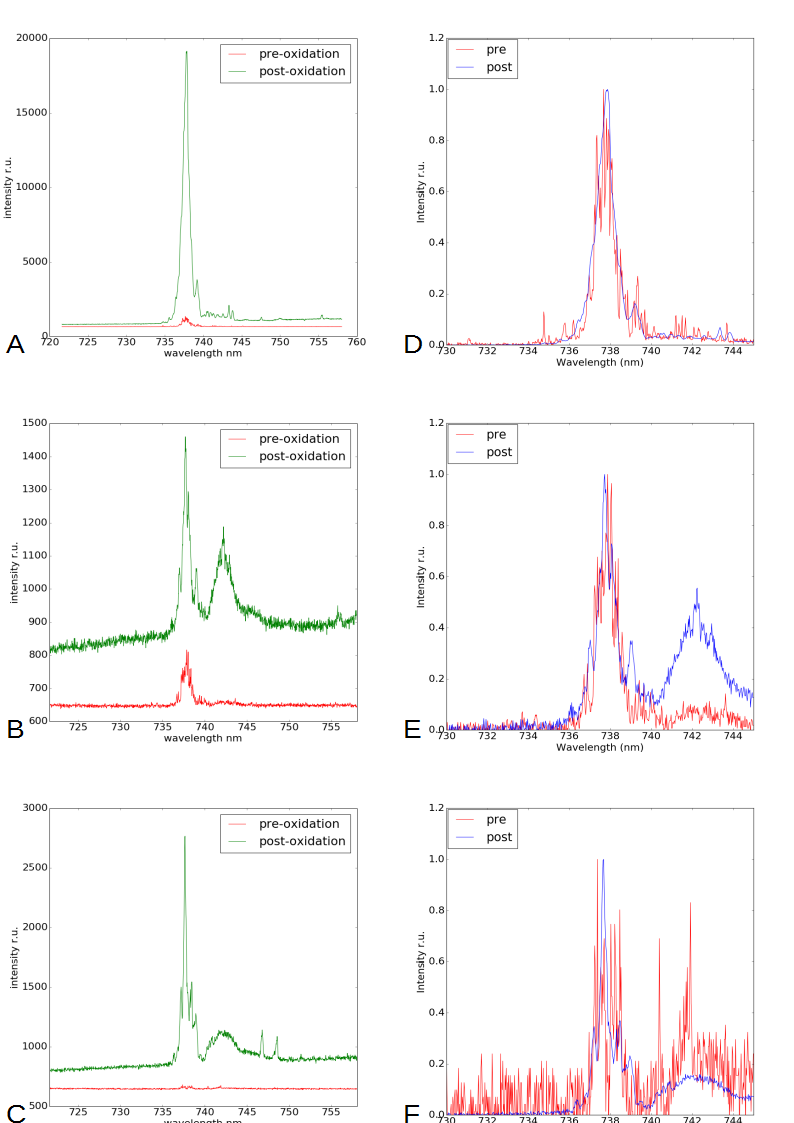
\includegraphics[width=1\linewidth]{Figures/pic/prepostoxidationspectra}
	\caption{Comparison between the PL Spectra of 3 of the pois from sample1508. Left column: real value. Right column: normalized spectra. The spectra were recorded with 120uW of excitation power with 532nm green laser and 1s of exposure time. A,D: ref4, B,E: ref3, C,F: ref5.}
	\label{fig:prepostoxidationspectra}
\end{figure}

\begin{figure}[h]
	\centering
	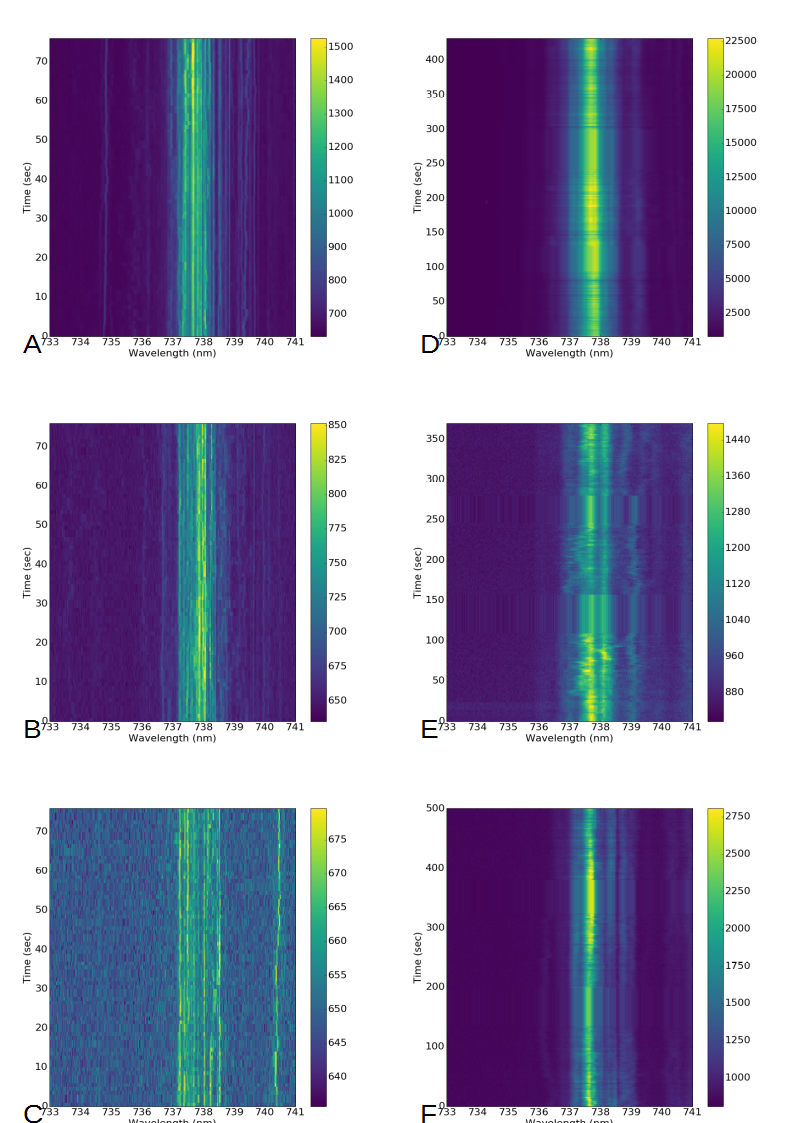
\includegraphics[width=1\linewidth]{Figures/pic/prepostoxidationtimeresolvespectra}
	\caption{The time-resolved spectra of pois from \ref{fig:prepostoxidationspectra}. The spectra were also recorded with 120uW of excitation power with 532nm green laser and 1s of exposure time. Left column: before oxidation, right column: after oxidation. A,D: ref4, B,E: ref3, C,F: ref5.The spectra were ploted in the order of real time, the stretched pixel is the blank for refocus.}
	\label{fig:prepostoxidationtimeresolvespectra}
\end{figure}

\begin{figure}[h]
	\centering
	\includegraphics[width=0.7\linewidth]{"Figures/pic/Histogram of normalized cross-correlation_2_o"}
	\caption{Histogram comparing the normalized mean value of cross-correlation between untreated and oxidized sample 1509(nanodiamond batch1) at 4.7K. The height of the bars are normalized by the integration over bins. }
	\label{fig:histogram-of-normalized-cross-correlation2o}
\end{figure}

\section{Hydrogen termination and Spectral stability}

Hydrogen terminated diamond surface posses negative electron affinity \citep{maier_electron_2001,ristein_electronic_2000,diederich_electron_1998} and is related to the depletion of NV centres in diamond \citep{stacey_depletion_2012}. After hydrogen plasma treatment on sample1512(nanodiamonds batch1) as mentioned in \ref{Chaper2.5}, time-resolved PL and excitation polarisation-resolved PL were recorded at 20K.

The time resolved pattern has been plotted out in \ref{fig:hydrogenterminationtimeresolve}, a visibly improvement in the spectral stability is shown. The comparison of mean cross-correlation of untreated nanodiamonds batch1 and hydrogenated ones can be found in \ref{fig:histogram-of-normalized-cross-correlation1h}, which agrees with the observation. As reference the comparison between nanodiamonds batch2 and hydrogen terminated batch1 was also plotted \ref{fig:histogram-of-normalized-cross-correlation1h2}. The hydrogenated nanodiamonds also responds the changes in excitation polarisation better. Clear polarisation dependency pattern can be seen in \ref{fig:hydrogenterminationpolarisation}. It has been noticed in the polarisation pattern of untreated nanodiamonds, that despite the general pattern reflects no polarisation dependency, some of the lines can still be seen changing periodically with the excitation polarisation. If we look closely at figure B and E in \ref{fig:hydrogenterminationpolarisation}, between 735nm and 737nm, there is a broader and less bright band whose not only intensity but also width changes with excitation polarisation. This pattern has also been seen in the pre-treatment sample.

\begin{figure}[h]
\centering
\includegraphics[width=0.7\linewidth]{"Figures/pic/Histogram of normalized cross-correlation_1_H"}
\caption{Histogram comparing the normalized mean value of cross-correlation between untreated sample 1510 and hydrogen plasma treated sample 1512 (both spin coated with nanodiamond from the batch1).The height of the bars are normalized by the integration over bins.  }
\label{fig:histogram-of-normalized-cross-correlation1h}
\end{figure}

\begin{figure}[h]
\centering
\includegraphics[width=0.7\linewidth]{"Figures/pic/Histogram of normalized cross-correlation_1_H_2"}
\caption{Histogram comparing the normalized mean value of cross-correlation between untreated sample 1508(nanodiamond batch2) and hydrogen plasma treated sample 1512(nanodiamond batch1).The height of the bars are normalized by the integration over bins.  }
\label{fig:histogram-of-normalized-cross-correlation1h2}
\end{figure}

\begin{figure}[h]
\centering
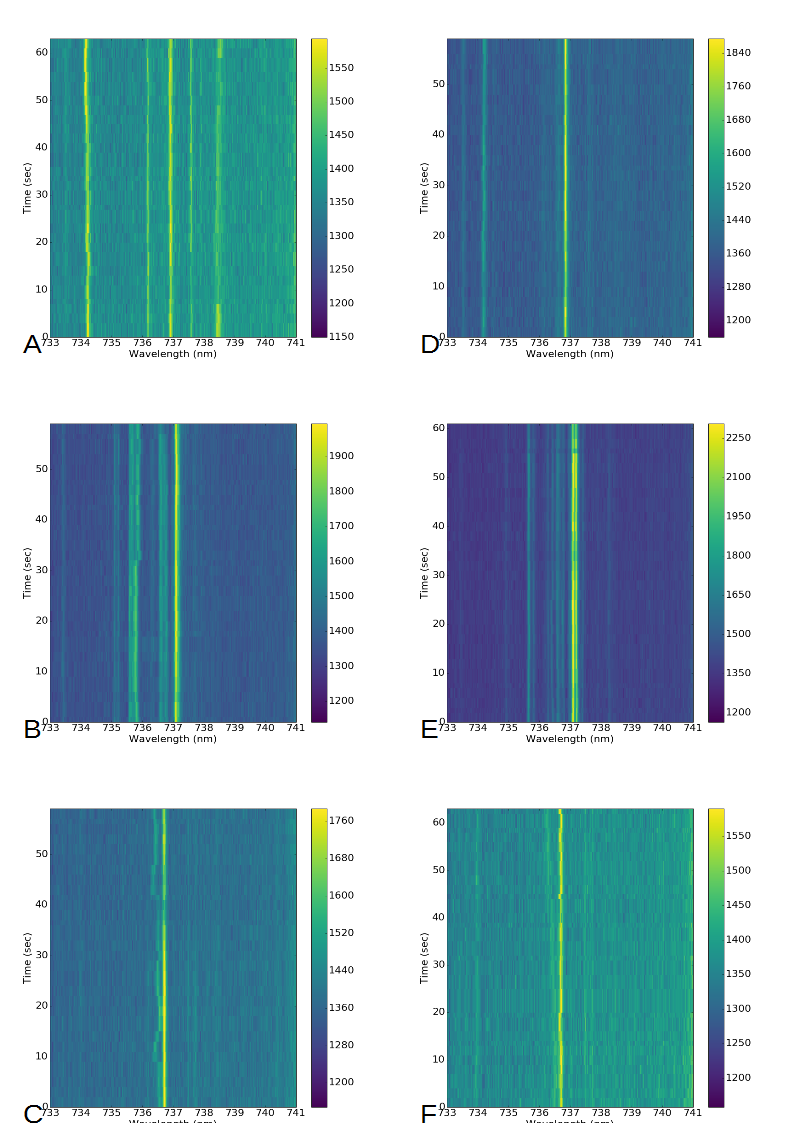
\includegraphics[width=1\linewidth]{Figures/pic/hydrogenterminationtimeresolve}
\caption{Time-resolved PL spectra of poi ref18, ref19 and ref20 from sample1512 at 20K. The excitation polarisation of left and right column are perpendicular to each other.
A,D: ref20, B,E: ref19, C,F: ref18}
\label{fig:hydrogenterminationtimeresolve}
\end{figure}

\begin{figure}[h]
\centering
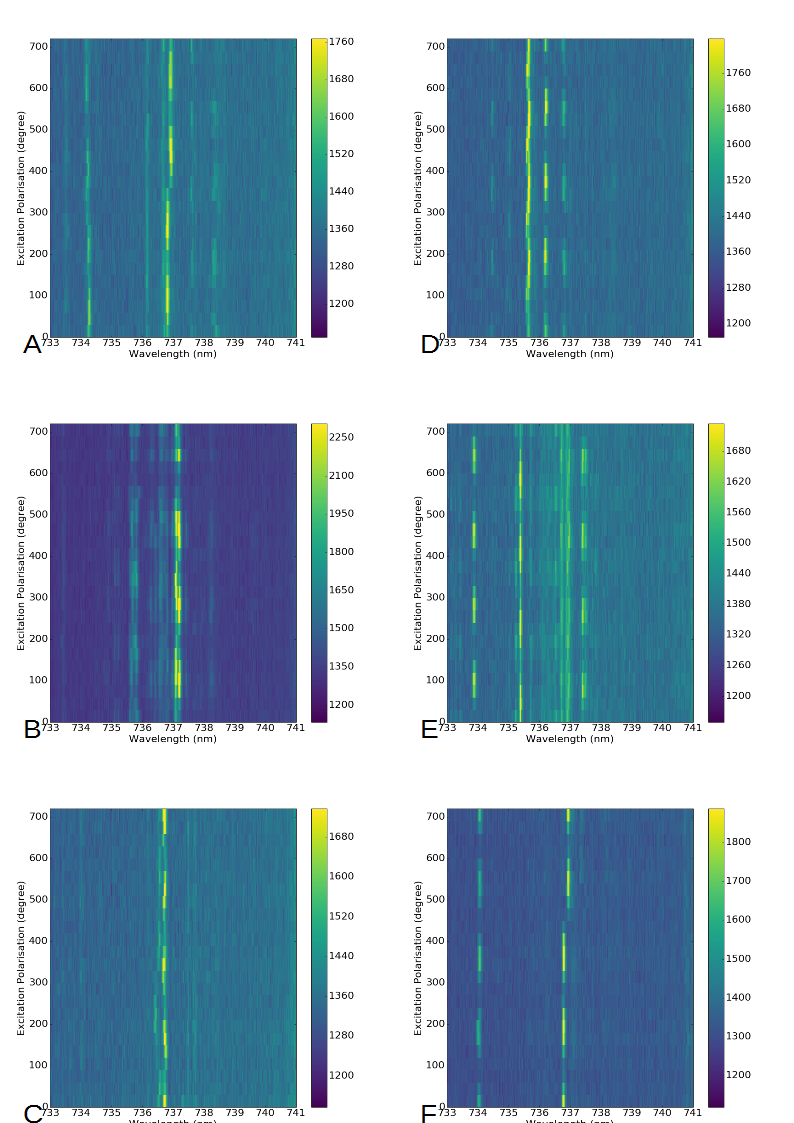
\includegraphics[width=1\linewidth]{Figures/pic/hydrogenterminationpolarisation}
\caption{The excitation polarisation-resolved spectra of pois from sample1512 at 20K. A: ref20, b:ref19, C:ref18, D:ref15, E:ref13, F:ref12.}
\label{fig:hydrogenterminationpolarisation}
\end{figure}



\section{Discussion}

The size effect of colour centre in nanodiamonds is often related the the surface band bending phenomena. There is higher chance for nanodiamonds from batch1, which are of smaller sizes, to obtain SiV$^{-}$s sitting inside the bended band than those ones of larger diameters, like the ones from batch2. In the paper \citep{rogers_multiple_2013}, SiV$^{-}$s in bulk diamond were reported to have very good long term spectral stability (no spectral position variation in 90min). Interestingly, the distance of SiV$^{-}$s from the surface was larger than 2um, which indicates SiV$^{-}$s sitting in the bulk diamond region instead of band bended region. 

As the samples are nitrogen doped, it is expected to have a upward band-bending, with a fermi level between the conduction band and the donor level. When the surface chemical potential is low enough, it is possible to have the donor level, even valence band maximum of the bulk region crossing the fermi level near the surface, which results in the accumulation of holes. 

The Nitrogen atom level lies 1.7eV below the minimum of the conduction band \citep{diederich_electron_1998}, at cryogenic temperature, the main electron source is the photon-excited electrons, with our 532nm excitation laser, it is not possible to excite electron from the valence band, but possible from the donor level.

\begin{figure}[h]
\centering
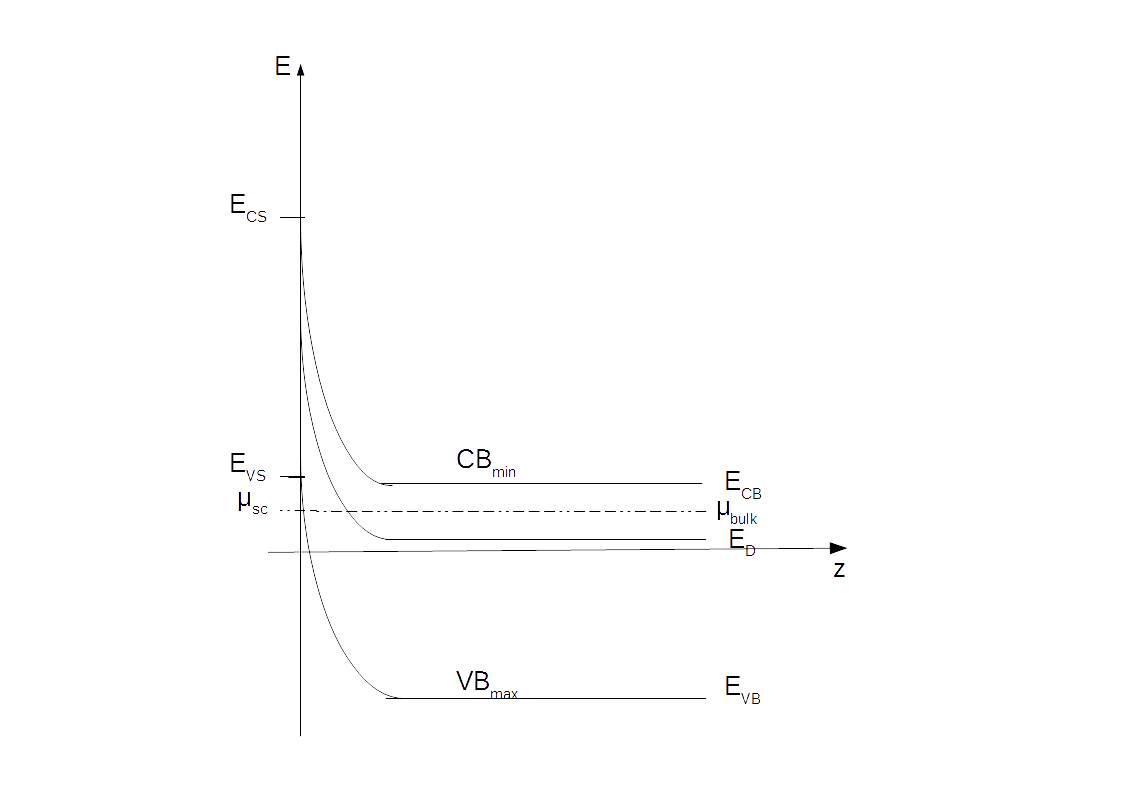
\includegraphics[width=1\linewidth]{Figures/pic/nbandbend}
\caption{Sketch of band bending in n doped nitrogen vacancy. The cross over of fermi level and nitrogen atom level may cause the accumulation of holes. E$_{D}$: donor level, the nitrogen atom level. E$_{CB}$: bulk conduction band minimum. E$_{VB}$: bulk valence band maximum. E$_{CS}$: surface conduction band minimum. E$_{VS}$: surface valence band maximum. $\mu_{SC}$: surface chemical potential. $\mu_{bulk}$: bulk chemical potential.} 
\label{fig:nbandbend}
\end{figure}
 

Since the accumulation of holes at the nitrogen atom level, the electrons from the conduction band are encouraged to recombine with the holes and emit photons. Since 1.7eV is already larger than the band gap between SiV$^{-}$ ground state and the first excited state, these spontaneous emission can be involved in the excitation of SiV$^{-}$s. 
While the polarisation of spontaneous emission is not relevant to the excitation polarisation, the excitation polarisation pattern of SiV$^{-}$ may not be solely the reflection of excitation polarisation but also the polarisation of spontaneous emission from the conduction band, which explains the patterns in \ref{fig:polarisationexcitation}.

As excitation power increases, more electrons are excited into the conduction band, which leads to further increase of spontaneous emission, which can be related to the power dependency of spectral diffusion in \ref{fig:powerdependencybeforeafteroxidation} and  \ref{fig:powerdependenceref11} that the spectral diffusion reduces as the power decreases.

It is assumed that the surface treatment alters the surface chemical potential and affects the depth of  the hole accumulating region. In \citep{stacey_depletion_2012} it is mentioned that the hydrogenation induced larger upward band bending in diamonds, while in \citep{diederich_electron_1998} the hydrogenated n-doped diamond had smaller upward band bending than the 'clean' one. This is because, the low surface potential in \citep{stacey_depletion_2012} is caused by adsorbent (water layer), while \citep{diederich_electron_1998} discussed adsorbent-free surfaces. Our sample is measure in UHV at cryogenic temperature, there shall be no water layer or other surface adsorbent involves, so we assume a reduced band bending is formed under the surface after hydrogenation, and this fits the measurement result. From the result it seems the aerobic oxidation has decreased the surface potential, which increases the band bending. The surface contaminations also affects the surface charge distribution, thus it is hard to tell if the observations are related to the surface contamination or not. More experiments need to be carried out for better understanding of the mechanism behind these phenomena. 





\chapter{Conclusion and outlook} % Main chapter title

\label{Chapter3} % Change X to a consecutive number; for referencing this chapter else where, use \ref{ChapterX}
%----------------------------------------------------------------------------------------
%	SECTION 1
%----------------------------------------------------------------------------------------

\section{Conclusion}

In the thesis we characterised spectrally the SiV$^{-}$ in nanodiamonds of 2 different size distributions with the help of confocal microscopy at cryogenic temperature. It has been noticed that the untreated SiV$^{-}$ in nanodiamonds are spectrally not stable, and SiV$^{-}$ smaller diamonds have worse spectral stability than larger ones. This spectral diffusion can be resolved in PL spectra. Previously it has been shown that the surface charging state plays a vital role in color centre luminescence. Negative charges on the surface can lead to depletion of NV \citep{stacey_depletion_2012}. For nanodiamonds, the band bending which originates from the difference of chemical potential in the bulk and on the surface is closely related to size-effect relating phenomena. It is highly suspected that the spectral diffusion of SiV$^{-}$ in nanodiamonds is also surface charge related.

Large number of PL spectra were taken to trace drift of lines. A standard method for spectral stability has been put forward. The calculation of mean cross-correlation can conclude the similarity of spectra into one number ranging from 0 to 1, Which makes statistical comparison possible. At the same time, time-resolved spectra realises the visualisation of spectra diffusion by plotting spectra over time in to colour maps.

Three surface treatment has been employed to modify the surface charging property. Aerobic Oxidation at 460$^{o}C$ - 480$^{o}C$ was used to selectively remove the graphitic defects on the surface while mild oxidation, resulting in carbonyl and carboxyl groups covered surface. Elevated temperature oxidation (575$^{o}C$) was used to initialize a bulk-diamond-like surface structure. Hydrogenation was to form a surface that posses negative electron affinity.

The oxidation at elevated temperature didn't produce useful data due to the distraction of substrate. The mildly oxidized sample showed heavily enhanced luminescence and worse spectral stability while the hydrogen terminated sample showed slightly reduced luminescence intensity and improved spectral stability.

%-----------------------------------
%	SECTION 2
%-----------------------------------
\section{ Outlook}

\paragraph{PL and PLE}
It is suspected that the ionization of Nitrogen atoms has been involved in the process, it is interested to compare the time-resolved spectra excited with a 532nm laser and a laser of 730nm.

PLE characterisation of the sample with improved spectra stability is also attractive, with reduced spectral diffusion, it might be finally possible for us to resolve the 4 line structure of SiV$^{-}$ ZPL.

\paragraph{life time measurement}
Due to the spectral diffusion, the orbital T1 measurement of untreated sample was not able to be carried out. With the improved spectral stability (need to be proved by PLE first), it might become possible. A longer time life will offers more possibility on the development of SiV$^{-}$ qubit.

\paragraph{Surface treatments}

Different surface treatments and comparison can help us understand the mechanism of spectral diffusion better. The most convenient treatments now are the hydroxylation which can be carried out directly on the hydrogenated sample resulting in a transform from negative electron affinity to positive electron affinity of the surface.

Anther interesting treatment is the dehydrogenation of sample by vacuum annealing, as the temperature varies, this can result in a clean diamond surface or a surface covered with thin-thick layer of graphite, which results in a gradual change in the surface electron affinity. \citep{diederich_electron_1998,maier_electron_2001}

Aerobic Oxidation still has more possibility to deal with. Since the size reduction rate of certain temperature is known, it is possible to profile the size effect on spectral stability by decreasing the size of nanodiamonds via oxidation gradually. It can also used to treat nanodiamonds that are too large (batch3, 4) for phonon elimination. The oxidation can also help to separate aggregated diamonds.

\paragraph{better method for size selection}
It is noticed, the size selection via centrifugation works, but is quite coarse. It might be possible to obtain finer batches by methods like high performance liquid chromatography. \citep{naoki_komatsu_chromatographic_2011}

\paragraph{relation between surface geometry and spectral behaviour}
Since it is possible to obtain the excitation polarisation pattern, it is interesting to observe the orientation preference of SiV$^{-}$/nanodiamonds statistically. This can be related to the formation process of HPHT diamond.




%----------------------------------------------------------------------------------------
%	THESIS CONTENT - APPENDICES
%----------------------------------------------------------------------------------------

\appendix % Cue to tell LaTeX that the following "chapters" are Appendices

% Include the appendices of the thesis as separate files from the Appendices folder
% Uncomment the lines as you write the Appendices

% Appendix A

\chapter{Appendix Title Here} % Main appendix title

\label{AppendixA} % For referencing this appendix elsewhere, use \ref{AppendixA}

Write your Appendix content here.
%\include{Appendices/AppendixB}
%\include{Appendices/AppendixC}

%----------------------------------------------------------------------------------------
%	BIBLIOGRAPHY
%----------------------------------------------------------------------------------------

\printbibliography[heading=bibintoc]

%----------------------------------------------------------------------------------------

\end{document}  
